\documentclass[12pt, a4paper]{article}

\usepackage[utf8]{inputenc}
\usepackage[T1]{fontenc}
\usepackage{lmodern}
\usepackage{fix-cm}

\usepackage[spanish]{babel}
\addto\captionsspanish{\renewcommand{\tablename}{Tabla}} 

\usepackage{amsmath, amssymb}
\usepackage{graphicx}
\usepackage{xcolor}


\usepackage{pgfplots}
\pgfplotsset{compat=1.18}

\usepackage{tikz}
\usetikzlibrary{shapes.geometric, arrows.meta, positioning}
\usepackage{geometry}
\usepackage{booktabs}
\usepackage{array}
\usepackage{fancyhdr}
\usepackage{float}
\usepackage{caption}
\usepackage{listings}
\usepackage{pdflscape}
\usepackage{multirow}
\usepackage{hyperref}

\geometry{margin=2cm, top=3cm, bottom=3cm}
\setlength{\headheight}{13.6pt}

% Configuración global de tablas
\renewcommand{\arraystretch}{1.2}
\captionsetup[table]{skip=8pt}

% Tipos de columna con salto de línea automático
\newcolumntype{L}[1]{>{\raggedright\arraybackslash}p{#1}}   % Izquierda con ancho
\newcolumntype{R}[1]{>{\raggedleft\arraybackslash}p{#1}}    % Derecha con ancho
\newcolumntype{C}[1]{>{\centering\arraybackslash}p{#1}}     % Centrado con ancho
\newcolumntype{J}[1]{>{\arraybackslash}p{#1}}               % Justificado con ancho

% Para tabularx (ancho flexible)
\newcolumntype{X}{>{\raggedright\arraybackslash}X}          
\newcolumntype{Y}{>{\centering\arraybackslash}X}            
\newcolumntype{Z}{>{\raggedleft\arraybackslash}X}         

% Entorno de tabla estándar
\newenvironment{mitabla}[2][H]{%
  \begin{table}[#1]
  \centering
  \caption{#2}
  \small
}{%
  \end{table}
}

\pagestyle{fancy}
\fancyhf{}
\rhead{\small Taller de Simulación de Sistemas}
\lhead{\small Informe de Actividad}
\cfoot{\thepage}
\renewcommand{\headrulewidth}{0.4pt}

\lstset{
  language=Java,
  basicstyle=\ttfamily\small,
  keywordstyle=\color{blue}\bfseries,
  commentstyle=\color{green!50!black},
  stringstyle=\color{red!60!black},
  numbers=left,
  numberstyle=\tiny\color{gray},
  frame=single,
  breaklines=true,
  tabsize=4,
  literate=
    {á}{{\'a}}1 {é}{{\'e}}1 {í}{{\'\i}}1 {ó}{{\'o}}1 {ú}{{\'u}}1
    {Á}{{\'A}}1 {É}{{\'E}}1 {Í}{{\'I}}1 {Ó}{{\'O}}1 {Ú}{{\'U}}1
    {ñ}{{\~n}}1 {Ñ}{{\~N}}1
}

\begin{document}

\setlength{\parindent}{0pt}

\begin{titlepage}
\centering
\begin{minipage}{\textwidth}
\end{minipage}
\begin{minipage}{\textwidth}
\centering
\large UNIVERSIDAD MAYOR DE SAN SIMÓN
\large FACULTAD DE CIENCIAS Y TECNOLOGÍA

\large INGENIERÍA DE SISTEMAS
\end{minipage}

\begin{minipage}{\textwidth}
\end{minipage}
\vspace{6cm}

{\huge Aplicaciones de Simulación de Sistemas}
\vfill 

\begin{flushleft}

Nombre: Miguel Mita Choque

Docente: Henrry Frank Villarroel Tapia

Materia: Taller de Simulación de Sistemas

\end{flushleft}

\end{titlepage}

\tableofcontents
\newpage

\setlength{\parskip}{10pt}

\section{Transformada Inversa}

\subsection{Introducción}

El método de Transformada Inversa es una de las tres técnicas vistas en la materia (junto con Rechazo y Composición) para generar valores de una variable aleatoria continua a partir de números aleatorios uniformes $0 < R < 1$. En este problema se aplica a una función $f(x)$ definida por tramos en el intervalo $[0,6]$.

\subsection{Descripción del problema}

La función proporcionada es:
\[
f(x)=\begin{cases}\dfrac{(x-3)^2}{18} &;\ 0 \leq x \leq 6 \\ 0 &;\ 0 > x > 6\end{cases}
\]

El objetivo consiste en generar valores aleatorios mediante el método de transformada inversa y verificar que los valores obtenidos pertenezcan al intervalo $[0,6]$.

Representación gráfica:

\begingroup
\tracinglostchars=0
\begin{figure}[H]
\centering
\begin{tikzpicture}
\begin{axis}[
  width=10cm, height=6cm,
  xlabel={$x$}, ylabel={$f(x)$},
  xmin=-0.5, xmax=6.5,
  ymin=-0.02, ymax=0.6,
  grid=both, grid style={line width=0.2pt, draw=gray!30},
  title={Función $f(x) = \frac{(x-3)^2}{18}$},
  xtick={0,1,2,3,4,5,6},
  samples=100
]
\addplot[blue!70!black, thick, domain=0:6] {(x-3)^2/18};
\addplot[dashed, gray] coordinates {(3,0) (3,0.5)};
\node[below] at (axis cs:3,0) {$x=3$ (mín.)};
\node[above right] at (axis cs:0,0.5) {$f(0)=f(6)=\frac{1}{2}$};
\end{axis}
\end{tikzpicture}
\caption{Gráfica de la función proporcionada. Nótese que el mínimo se alcanza en $x=3$ y los valores máximos en los extremos $x=0$ y $x=6$.}
\end{figure}
\endgroup

\subsection{Propuesta de solución}

Se aplica el método de Transformada Inversa, que requiere seguir los siguientes cinco pasos:

\textbf{Paso 1: Contar con la función $f(x)$}

Sea $f(x)$:
\[
f(x)=\begin{cases}\dfrac{(x-3)^2}{18} &;\ 0 \leq x \leq 6 \\ 0 &;\ 0 > x > 6\end{cases}
\]

\textbf{Paso 2: Determinar la función acumulada}

Calculamos la función de distribución acumulada $F(x)$ integrando $f(x)$:
\[F(x) = \int_0^x \frac{(x-3)^2}{18}\, dx\]

Desarrollo:
\begin{align*}
F(x) &= \frac{1}{18} \int_0^x (x-3)^2\, dx \\[4pt]
     &= \frac{1}{18} \left[\frac{(x-3)^3}{3}\right]_0^x \\[4pt]
     &= \frac{1}{18} \left(\frac{(x-3)^3}{3} - \frac{(0-3)^3}{3}\right) \\[4pt]
     &= \frac{1}{18} \left(\frac{(x-3)^3}{3} + \frac{27}{3}\right) \\[4pt]
     &= \frac{1}{18} \cdot \frac{(x-3)^3 + 27}{3}
\end{align*}

\[
\boxed{F(x) = \frac{(x-3)^3 + 27}{54}}, \quad 0 \leq x \leq 6
\]

\textbf{Paso 3: Igualar la función acumulada}

Igualamos la función acumulada $F(x)$ con un número aleatorio $R$:
\[F(x) = R\]

Sustituyendo la expresión de $F(x)$:
\[\frac{(x-3)^3 + 27}{54} = R\]

\textbf{Paso 4: Aplicar función inversa}

Despejamos $x = F^{-1}(R)$ de la ecuación anterior:

\begin{align*}
\frac{(x-3)^3 + 27}{54} &= R \\[4pt]
(x-3)^3 + 27 &= 54R \\[4pt]
(x-3)^3 &= 54R - 27 \\[4pt]
x - 3 &= \sqrt[3]{54R - 27} \\[4pt]
x &= 3 + \sqrt[3]{54R - 27}
\end{align*}

\[
x=\begin{cases}3+\sqrt[3]{54R-27} &;\ 0 \leq R \leq 1 \\ 0 &;\ 0 > R > 1\end{cases}
\]

\subsection{Objetivos}

\textbf{Objetivo general:} Aplicar el método de Transformada Inversa para generar valores aleatorios de la variable $x$ con función de densidad $f(x)=\dfrac{(x-3)^2}{18}$.

\textbf{Objetivos específicos:}
\begin{enumerate}
    \item Obtener la función inversa $x = F^{-1}(R)$ a partir de la función acumulada $F(x)$.
    \item Validar mediante prueba de escritorio que los valores generados pertenecen al intervalo $[0,6]$.
\end{enumerate}

\subsection{Desarrollo de la solución}

\subsubsection{Algoritmo}

Del modelamiento se obtiene la propuesta algorítmica para generar la variable aleatoria $x$:

\begin{lstlisting}[caption={Algoritmo — Generación de variable aleatoria}, language=Pascal]
real funcion variableTransformadaInversa(real R){
    real x;
    x <- 3 + RaizCubica(54*R - 27);
    retornar x;
}
\end{lstlisting}

La función recibe un número aleatorio $0 < R < 1$ y retorna $x$ aplicando directamente la transformada inversa $x = 3 + \sqrt[3]{54R - 27}$ obtenida en el Paso 4 de la propuesta de solución.

\subsubsection{Diagrama de flujo}

\begin{figure}[H]
\centering
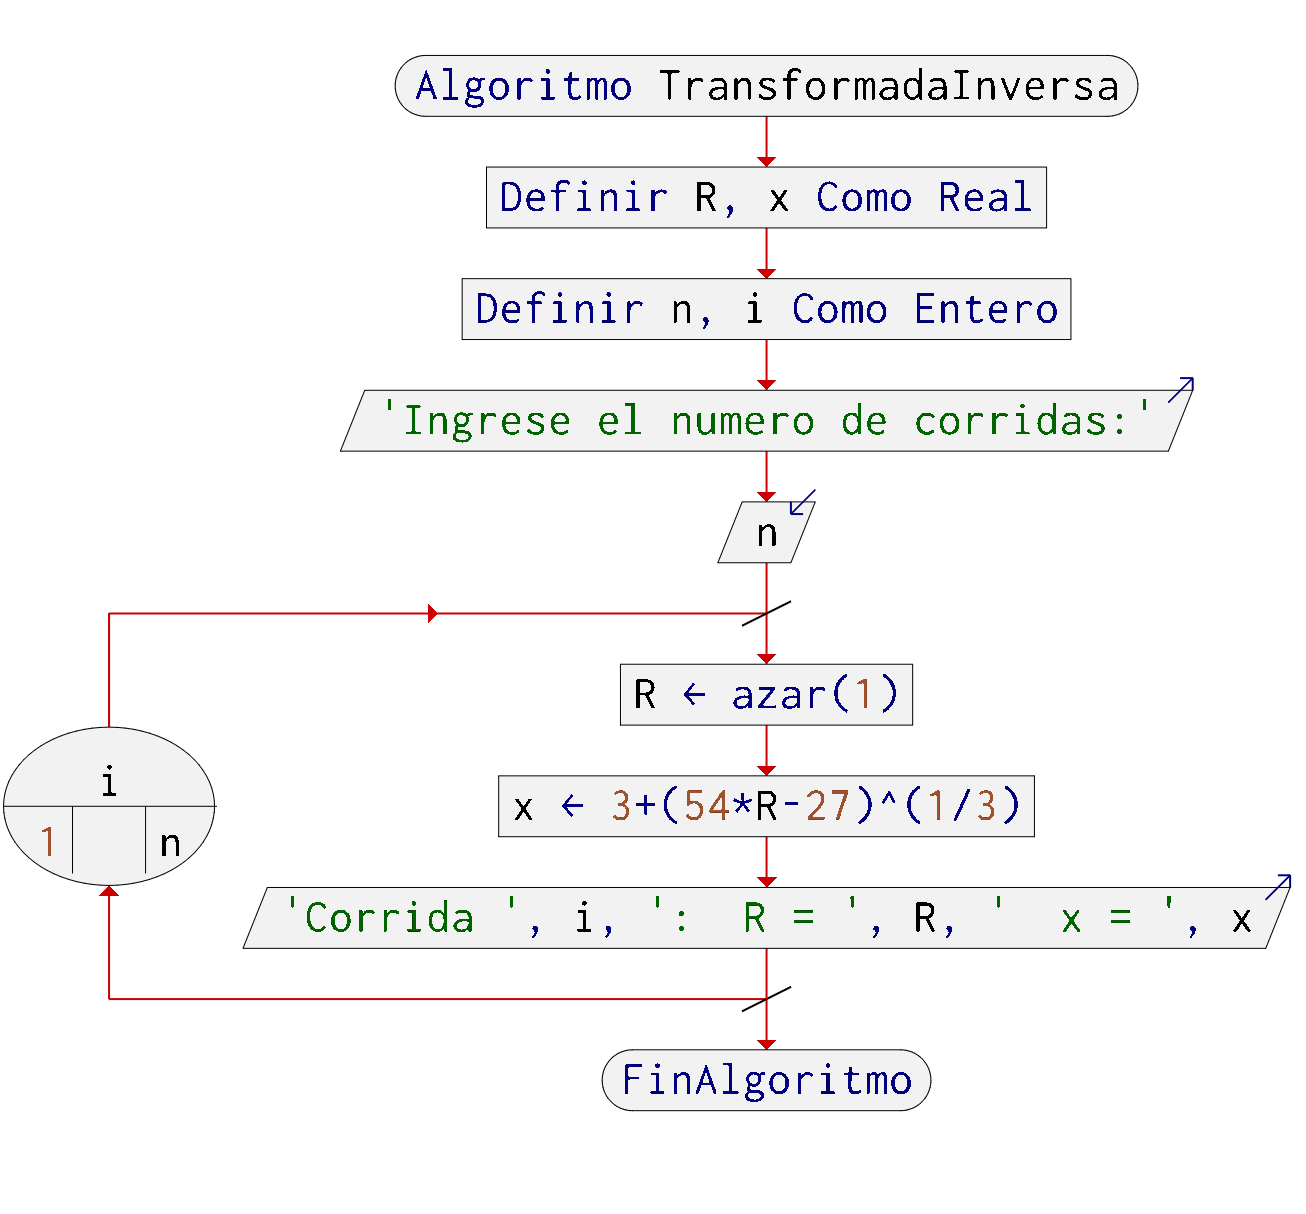
\includegraphics[width=0.8\textwidth]{capturas_pseint/p1_transformada_inversa.png}
\caption{Diagrama de flujo — Transformada Inversa (PSeInt)}
\end{figure}

\subsubsection{Tabla de simulación}

Cada fila es una corrida; cada columna es un paso del algoritmo:

\begin{mitabla}[H]{Tabla de simulación con $n=10$}
\begin{tabular}{c cc}
\toprule
Corrida & $R \leftarrow \text{gcm}()$ & $x = 3+\sqrt[3]{54R-27}$ \\
\midrule
1  & 0,9709 & $3+\sqrt[3]{54(0{,}9709)-27} = 5{,}9406$ \\
2  & 0,6970 & $3+\sqrt[3]{54(0{,}6970)-27} = 5{,}1994$ \\
3  & 0,3014 & $3+\sqrt[3]{54(0{,}3014)-27} = 0{,}7947$ \\
4  & 0,9728 & $3+\sqrt[3]{54(0{,}9728)-27} = 5{,}9445$ \\
5  & 0,8182 & $3+\sqrt[3]{54(0{,}8182)-27} = 5{,}5806$ \\
6  & 0,4939 & $3+\sqrt[3]{54(0{,}4939)-27} = 3{,}9563$ \\
7  & 0,7423 & $3+\sqrt[3]{54(0{,}7423)-27} = 5{,}2956$ \\
8  & 0,1593 & $3+\sqrt[3]{54(0{,}1593)-27} = 1{,}4297$ \\
9  & 0,0821 & $3+\sqrt[3]{54(0{,}0821)-27} = 0{,}6372$ \\
10 & 0,5821 & $3+\sqrt[3]{54(0{,}5821)-27} = 4{,}6902$ \\
\bottomrule
\end{tabular}
\end{mitabla}

\subsubsection{Implementación}

\begin{mitabla}[H]{Variables del modelamiento}
\begin{tabular}{cL{8cm}c}
\toprule
Variable & Descripción & Paso \\
\midrule
$R$ & Número aleatorio uniforme $0 < R < 1$, generado con \texttt{random()} & Paso 3 \\
$x$ & Variable aleatoria: $x = 3 + \sqrt[3]{54R - 27}$ & Paso 4 \\
\bottomrule
\end{tabular}
\end{mitabla}

\textbf{Implementación en Java:}

\begin{lstlisting}[caption={TransformadaInversa.java}, language=Java]
import java.util.Scanner;

public class TransformadaInversa {

    public static double generarX() {
        double R = Math.random();
        double x = 3 + Math.cbrt(54 * R - 27);
        return x;
    }

    public static void main(String[] args) {
        Scanner sc = new Scanner(System.in);
        System.out.print("Ingrese el numero de corridas n: ");
        int n = sc.nextInt();

        System.out.println("\nCorrida\tR\t\tx");
        for (int i = 1; i <= n; i++) {
            double R = Math.random();
            double x = 3 + Math.cbrt(54 * R - 27);
            System.out.printf("%d\t%.4f\t\t%.4f%n", i, R, x);
        }
        sc.close();
    }
}
\end{lstlisting}

\textbf{Implementación en Excel:}

\begin{figure}[H]
\centering
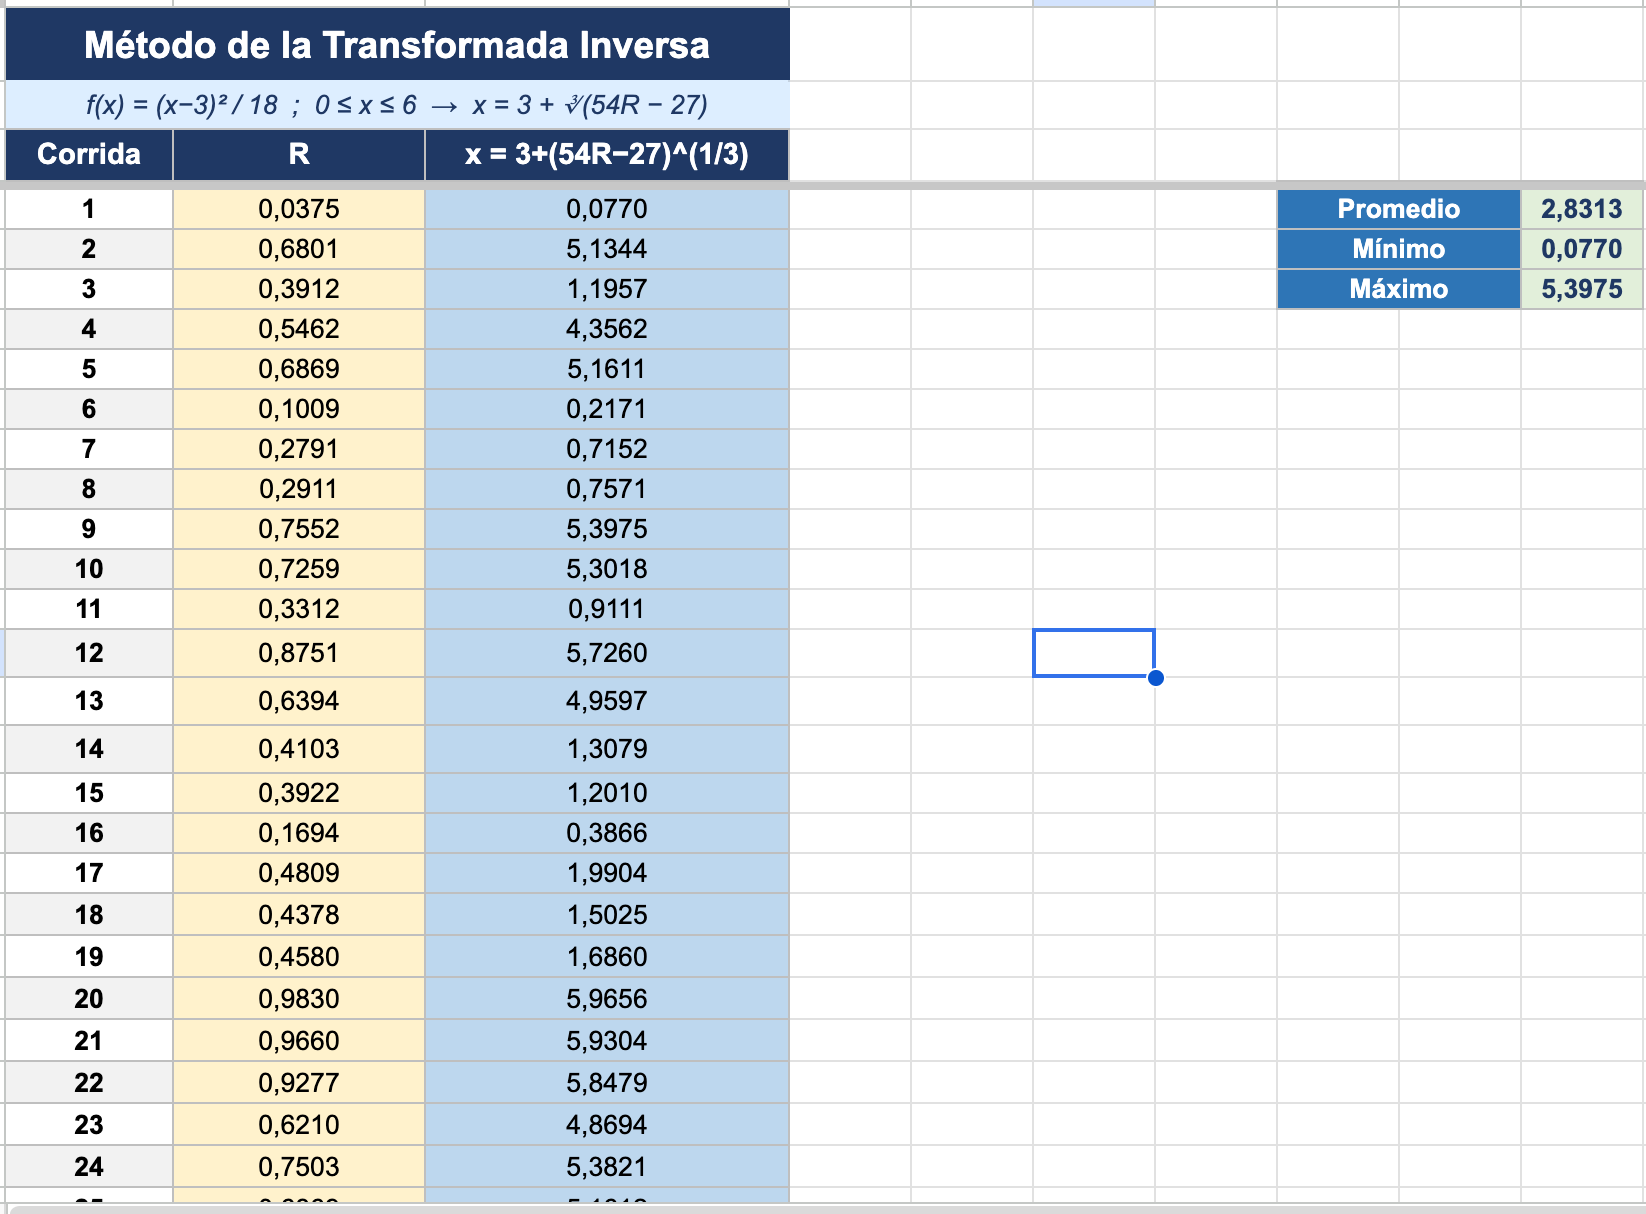
\includegraphics[width=0.9\textwidth]{capturas_excel/p1_transformada_inversa.png}
\caption{Hoja de cálculo — Transformada Inversa}
\end{figure}

\subsection{Validación}

\subsubsection{\texorpdfstring{Prueba de escritorio con $n=25$}{Prueba de escritorio con n=25}}

\begin{mitabla}[H]{\texorpdfstring{Validación con $n=25$ corridas}{Validacion con n=25 corridas}}
\begin{tabular}{ccc}
\toprule
Corrida & $R$ & $x=3+\sqrt[3]{54R-27}$ \\
\midrule
1 & 0,9663 & $3+\sqrt[3]{54(0,9663)-27} = 5,9311$ \\
2 & 0,3438 & $3+\sqrt[3]{54(0,3438)-27} = 0,9644$ \\
3 & 0,3865 & $3+\sqrt[3]{54(0,3865)-27} = 1,1702$ \\
4 & 0,8691 & $3+\sqrt[3]{54(0,8691)-27} = 5,7112$ \\
5 & 0,6990 & $3+\sqrt[3]{54(0,6990)-27} = 5,2067$ \\
6 & 0,9047 & $3+\sqrt[3]{54(0,9047)-27} = 5,7958$ \\
7 & 0,5043 & $3+\sqrt[3]{54(0,5043)-27} = 3,6150$ \\
8 & 0,8624 & $3+\sqrt[3]{54(0,8624)-27} = 5,6948$ \\
9 & 0,1001 & $3+\sqrt[3]{54(0,1001)-27} = 0,2153$ \\
10 & 0,8215 & $3+\sqrt[3]{54(0,8215)-27} = 5,5894$ \\
11 & 0,5857 & $3+\sqrt[3]{54(0,5857)-27} = 4,6667$ \\
12 & 0,6718 & $3+\sqrt[3]{54(0,6718)-27} = 5,1012$ \\
13 & 0,9590 & $3+\sqrt[3]{54(0,9590)-27} = 5,9157$ \\
14 & 0,4151 & $3+\sqrt[3]{54(0,4151)-27} = 1,3387$ \\
15 & 0,3255 & $3+\sqrt[3]{54(0,3255)-27} = 0,8878$ \\
16 & 0,1749 & $3+\sqrt[3]{54(0,1749)-27} = 0,4010$ \\
17 & 0,8745 & $3+\sqrt[3]{54(0,8745)-27} = 5,7245$ \\
18 & 0,1367 & $3+\sqrt[3]{54(0,1367)-27} = 0,3030$ \\
19 & 0,6410 & $3+\sqrt[3]{54(0,6410)-27} = 4,9674$ \\
20 & 0,7793 & $3+\sqrt[3]{54(0,7793)-27} = 5,4706$ \\
21 & 0,0548 & $3+\sqrt[3]{54(0,0548)-27} = 0,1138$ \\
22 & 0,2243 & $3+\sqrt[3]{54(0,2243)-27} = 0,5401$ \\
23 & 0,1344 & $3+\sqrt[3]{54(0,1344)-27} = 0,2974$ \\
24 & 0,7730 & $3+\sqrt[3]{54(0,7730)-27} = 5,4520$ \\
25 & 0,8552 & $3+\sqrt[3]{54(0,8552)-27} = 5,6769$ \\
\bottomrule
\end{tabular}
\end{mitabla}

\subsubsection{\texorpdfstring{Corridas con $n \geq 50$}{Corridas con n mayor igual 50}}

Para validar el comportamiento del algoritmo con muestras más grandes, se ejecutaron corridas con $n = 50$, $100$, $250$, $500$, $1000$. Se muestra el último valor generado en cada corrida:

\begin{mitabla}{\texorpdfstring{Resumen de corridas con $n \geq 50$}{Resumen de corridas con n mayor igual 50}}
\begin{tabular}{ccc}
\toprule
$n$ & $R$ (última corrida) & $x=3+\sqrt[3]{54R-27}$ \\
\midrule
50 & 0,7999 & $3+\sqrt[3]{54(0,7999)-27} = 4,3196$ \\
100 & 0,1036 & $3+\sqrt[3]{54(0,1036)-27} = 0,5612$ \\
250 & 0,0323 & $3+\sqrt[3]{54(0,0323)-27} = 0,1749$ \\
500 & 0,1626 & $3+\sqrt[3]{54(0,1626)-27} = 0,8788$ \\
1000 & 0,0629 & $3+\sqrt[3]{54(0,0629)-27} = 0,3430$ \\
\bottomrule
\end{tabular}
\end{mitabla}

\subsection{Interpretación}

\subsubsection{Resultados}

En las 25 corridas de la prueba de escritorio, todos los valores de $x$ generados quedaron dentro del intervalo $[0,6]$ esperado, con valores más frecuentes hacia los extremos del intervalo y menor densidad cerca de $x=3$, lo cual es consistente con la forma de $f(x)$ (mínimo en $x=3$, máximos en $x=0$ y $x=6$). Las corridas con $n \geq 50$ mantienen el mismo comportamiento al aumentar el tamaño de muestra.

\subsubsection{Interpretación}

Los resultados confirman que la función inversa $x = 3 + \sqrt[3]{54R-27}$ obtenida en la propuesta de solución genera correctamente valores de la variable aleatoria $x$ según la densidad $f(x) = \frac{(x-3)^2}{18}$: ningún valor generado cae fuera de $[0,6]$, y la mayor concentración de valores en los extremos coincide con las zonas de mayor densidad de la función.

\subsection{Conclusión}

El método de Transformada Inversa permitió obtener una función cerrada $x=F^{-1}(R)$ a partir de la función de densidad dada, la cual se validó mediante prueba de escritorio (n=25 y $n \geq 50$) y se implementó tanto en Java como en Excel, obteniendo en ambos casos resultados consistentes con el modelo teórico.


\newpage

\section{Composición}

\subsection{Introducción}

El método de Composición se aplica cuando la función de densidad puede dividirse en subfunciones $f_i(x)$ ponderadas por subáreas $A_i$; internamente cada subfunción se resuelve con Transformada Inversa. En este problema se aplica a una distribución triangular simbólica definida por los parámetros $a$, $b$, $c$.

\subsection{Descripción del problema}

\begin{quote}
Se tiene la siguiente distribución triangular en $[a,c]$ con vértice en $b$:
\end{quote}

\begin{center}
\shorthandoff{>}
\begin{tikzpicture}[scale=1.2]
  \draw[->] (0,0) -- (8,0) node[right] {$x$};
  \draw[->] (0,0) -- (0,4) node[above] {$f(x)$};
  \draw (1.5,0) -- (4,3) -- (6.5,0);
  \draw[dashed] (4,0) -- (4,3);
  \node[below] at (1.5,0) {$a$};
  \node[below] at (4,0)   {$b$};
  \node[below] at (6.5,0) {$c$};
\end{tikzpicture}
\shorthandon{>}
\end{center}

\[
f(x)=\begin{cases}
\dfrac{2(x-a)}{(b-a)(c-a)} &;\ a \leq x \leq b \\[8pt]
\dfrac{2(c-x)}{(c-a)(c-b)} &;\ b \leq x \leq c
\end{cases}
\]

\subsection{Propuesta de solución}

Se aplica el método de Composición, que requiere seguir los siguientes pasos.

\textbf{Paso 1: Contar con la función $f(x)$ y dividirla en subáreas}

\[
f(x) = \sum_{i=1}^{n} f_i(x) \cdot A_i \qquad ; \qquad \sum_{i=1}^{n} A_i = 1
\]

Determinando la altura $h$ de modo que $A_1 + A_2 = 1$:
\[
\tfrac{1}{2}(b-a)\cdot h + \tfrac{1}{2}(c-b)\cdot h = 1
\]
\[
\tfrac{h}{2}\big((b-a)+(c-b)\big) = 1
\]
\[
\tfrac{h}{2}(c-a) = 1
\]
\[
h = \frac{2}{c-a}
\]

Determinando subárea $A_1$:
\[
A_1 = \tfrac{1}{2}(b-a)\cdot\frac{2}{c-a} = \frac{b-a}{c-a}
\]

Determinando subárea $A_2$:
\[
A_2 = \tfrac{1}{2}(c-b)\cdot\frac{2}{c-a} = \frac{c-b}{c-a}
\]

\textbf{Paso 2: Definir las subfunciones $f_i(x)$}

Para la 1ra parte ($A_1'=1$), definida por los puntos $(a,0)$ y $(b,h_1)$:
\[
A_1' = \tfrac{1}{2}(b-a)\,h_1 = 1 \implies h_1 = \frac{2}{b-a}
\]
Ecuación de la recta:
\[
\frac{y - 0}{\dfrac{2}{b-a} - 0} = \frac{x - a}{b - a}
\]
\[
f_1(x) = \frac{2(x-a)}{(b-a)^2} \qquad ;\ a \leq x \leq b
\]

Para la 2da parte ($A_2'=1$), definida por los puntos $(b,h_2)$ y $(c,0)$:
\[
A_2' = \tfrac{1}{2}(c-b)\,h_2 = 1 \implies h_2 = \frac{2}{c-b}
\]
Ecuación de la recta:
\[
\frac{y - 0}{\dfrac{2}{c-b} - 0} = \frac{x - c}{b - c}
\]
\[
f_2(x) = \frac{-2(x-c)}{(c-b)^2} \qquad ;\ b \leq x \leq c
\]

\textbf{Paso 3: Reexpresar $f(x)$ en términos de $f_i(x)$ y $A_i$}

\[
f(x) = \frac{2(x-a)}{(b-a)^2}\cdot\frac{b-a}{c-a} + \frac{-2(x-c)}{(c-b)^2}\cdot\frac{c-b}{c-a}
\]
\[
f(x) = \frac{2(x-a)}{(b-a)(c-a)} - \frac{2(x-c)}{(c-b)(c-a)}
\]

Verificación: $A_1+A_2 = \dfrac{b-a}{c-a}+\dfrac{c-b}{c-a} = \dfrac{c-a}{c-a} = 1$ \checkmark

\textbf{Paso 4: Generar números aleatorios}

\[
R_1 \leftarrow \text{gcm}() \qquad ; \qquad R_2 \leftarrow \text{gcm}()
\]

\textbf{Paso 5: Relación entre acumuladas de área y subfunciones}

\[
\text{si } R_1 < A_1 = \frac{b-a}{c-a} \implies \text{escoger } f_1(x)
\]
\[
\text{si } R_1 \geq A_1 \implies \text{escoger } f_2(x)
\]

\textbf{Paso 6: Escoger subfunción con $R_1$}

\begin{lstlisting}[caption={Selección de subfunción}, language=Pascal]
si (R1 < (b-a)/(c-a))
    escoger f1(x)
sino
    escoger f2(x)
fin si
\end{lstlisting}

\textbf{Paso 7: Aplicar Transformada Inversa a la subfunción escogida}

\textit{Aplicando TI a la subfunción $f_1(x)$:}

\textbf{Paso 1.} Sea $f_1(x)$:
\[
f_1(x) = \frac{2(x-a)}{(b-a)^2} \qquad ;\ a \leq x \leq b
\]

\textbf{Paso 2.} Determinar la función acumulada $F_1(x)$:
\[
F_1(x) = \int_a^x \frac{2(x-a)}{(b-a)^2}\,dx = \frac{2}{(b-a)^2} \int_a^x (x-a)\,dx
\]
Aplicando la regla de la potencia:
\[
F_1(x) = \frac{2}{(b-a)^2} \left[\frac{(x-a)^2}{2}\right]_a^x = \frac{2}{(b-a)^2}\cdot\frac{(x-a)^2}{2}
\]
\[
\boxed{F_1(x) = \frac{(x-a)^2}{(b-a)^2}} \qquad ;\ a \leq x \leq b
\]

\textbf{Paso 3.} Igualar $F_1(x) = R_2$:
\[
\frac{(x-a)^2}{(b-a)^2} = R_2
\]

\textbf{Paso 4.} Aplicar función inversa:
\[
(x-a)^2 = (b-a)^2\,R_2
\]
\[
x - a = (b-a)\sqrt{R_2}
\]
\[
x_1=\begin{cases}a+(b-a)\sqrt{R_2} &;\ 0 \leq R_2 \leq 1 \\ 0 &;\ 0 > R_2 > 1\end{cases}
\]

\textit{Aplicando TI a la subfunción $f_2(x)$:}

\textbf{Paso 1.} Sea $f_2(x)$:
\[
f_2(x) = \frac{-2(x-c)}{(c-b)^2} \qquad ;\ b \leq x \leq c
\]

\textbf{Paso 2.} Determinar la función acumulada $F_2(x)$:
\[
F_2(x) = \int_b^x \frac{-2(x-c)}{(c-b)^2}\,dx = \frac{-2}{(c-b)^2} \int_b^x (x-c)\,dx
\]
Aplicando la regla de la potencia:
\[
F_2(x) = \frac{-2}{(c-b)^2}\left[\frac{(x-c)^2}{2}\right]_b^x = \frac{-2}{(c-b)^2}\cdot\left(\frac{(x-c)^2}{2} - \frac{(b-c)^2}{2}\right)
\]
Expandiendo $(b-c)^2 = (b-c)(b-c) = b^2-2bc+c^2 = (c-b)^2$:
\[
F_2(x) = \frac{-2}{(c-b)^2}\cdot\frac{(x-c)^2-(c-b)^2}{2} = \frac{-(x-c)^2+(c-b)^2}{(c-b)^2}
\]
\[
\boxed{F_2(x) = 1 - \frac{(x-c)^2}{(c-b)^2}} \qquad ;\ b \leq x \leq c
\]

\textbf{Paso 3.} Igualar $F_2(x) = R_2$:
\[
1 - \frac{(x-c)^2}{(c-b)^2} = R_2 \implies \frac{(x-c)^2}{(c-b)^2} = 1-R_2
\]

\textbf{Paso 4.} Aplicar función inversa:
\[
(x-c)^2 = (c-b)^2(1-R_2)
\]
Como $b \leq x \leq c$ entonces $x-c \leq 0$, se toma la raíz negativa:
\[
x-c = -(c-b)\sqrt{1-R_2}
\]
\[
x_2=\begin{cases}c-(c-b)\sqrt{1-R_2} &;\ 0 \leq R_2 \leq 1 \\ 0 &;\ 0 > R_2 > 1\end{cases}
\]

La variable final por composición:
\[
x=\begin{cases}
x_1 = a+(b-a)\sqrt{R_2}   & ;\ R_1 < \dfrac{b-a}{c-a} \\[8pt]
x_2 = c-(c-b)\sqrt{1-R_2} & ;\ R_1 \geq \dfrac{b-a}{c-a}
\end{cases}
\]

\textbf{Paso 8: Repetir para el tamaño de muestra requerido}

Se repiten los pasos anteriores para generar las observaciones necesarias de la simulación.

\subsection{Objetivos}

\textbf{Objetivo general:} Aplicar el método de Composición (con Transformada Inversa) para generar valores aleatorios de una variable con distribución triangular en $[a,c]$.

\textbf{Objetivos específicos:}
\begin{enumerate}
    \item Determinar las subfunciones $f_1(x)$, $f_2(x)$ y sus subáreas $A_1$, $A_2$ mediante el método de composición.
    \item Validar mediante prueba de escritorio que los valores generados se ajustan al rango $[a,c]$ y a la proporción esperada entre subfunciones.
\end{enumerate}

\subsection{Desarrollo de la solución}

\subsubsection{Algoritmo}

Del modelamiento se obtiene la propuesta algorítmica para generar la variable aleatoria $x$:

\begin{lstlisting}[caption={Pseudocódigo — Método de Composición}, language=Pascal]
FUNCION variableComposicion() : Real
    DEFINIR R1, R2, x : Real
    R1 <- gcm()
    R2 <- gcm()
    SI R1 < (b-a)/(c-a) ENTONCES
        x <- a + (b-a) * raiz(R2)
    SINO
        x <- c - (c-b) * raiz(1-R2)
    FIN SI
    Retornar x
FIN FUNCION
\end{lstlisting}

\subsubsection{Diagrama de flujo}

\begin{figure}[H]
\centering
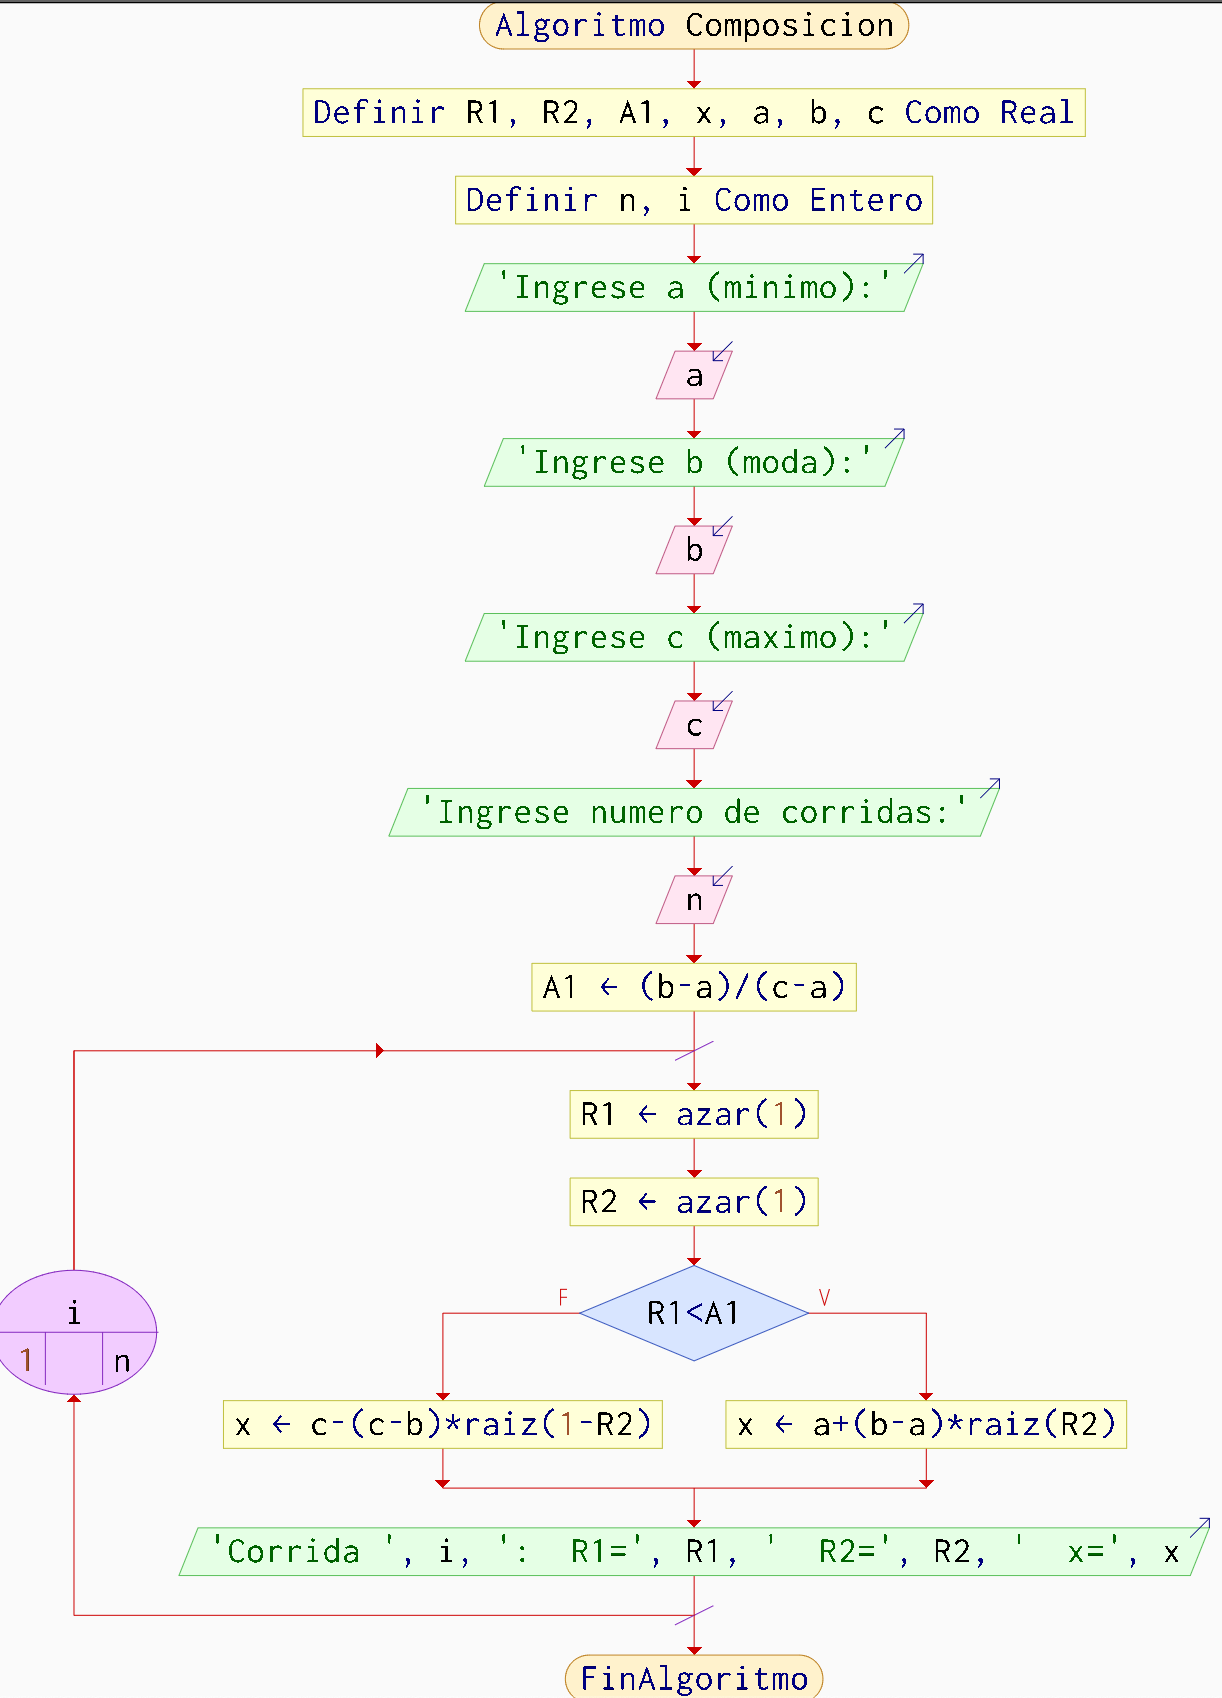
\includegraphics[width=0.5\textwidth]{capturas_pseint/p2_composicion.png}
\caption{Diagrama de flujo — Composición (PSeInt)}
\end{figure}

\subsubsection{Tabla de simulación}

Con $a=1{,}5$, $b=4$, $c=6{,}5$ y $A_1=\dfrac{b-a}{c-a}=0{,}5$.
Cada fila es una corrida; cada columna es un paso del algoritmo:

\begin{mitabla}[H]{Tabla de simulación con $n=10$}
\small
\begin{tabular}{c c c c L{5.5cm}}
\toprule
Corrida & $R_1 \leftarrow \text{gcm}()$ & $R_2 \leftarrow \text{gcm}()$ & Sub & $x$ \\
\midrule
1  & 0,9077 & 0,5115 & $f_2$ & $6{,}5-2{,}5\sqrt{1-0{,}5115}=4{,}7527$ \\
2  & 0,2128 & 0,0785 & $f_1$ & $1{,}5+2{,}5\sqrt{0{,}0785}=2{,}2005$ \\
3  & 0,4475 & 0,7656 & $f_1$ & $1{,}5+2{,}5\sqrt{0{,}7656}=3{,}6875$ \\
4  & 0,6524 & 0,7491 & $f_2$ & $6{,}5-2{,}5\sqrt{1-0{,}7491}=5{,}2478$ \\
5  & 0,4321 & 0,6206 & $f_1$ & $1{,}5+2{,}5\sqrt{0{,}6206}=3{,}4694$ \\
6  & 0,7857 & 0,5601 & $f_2$ & $6{,}5-2{,}5\sqrt{1-0{,}5601}=4{,}8419$ \\
7  & 0,3858 & 0,2163 & $f_1$ & $1{,}5+2{,}5\sqrt{0{,}2163}=2{,}6627$ \\
8  & 0,7241 & 0,1473 & $f_2$ & $6{,}5-2{,}5\sqrt{1-0{,}1473}=4{,}1915$ \\
9  & 0,6775 & 0,1335 & $f_2$ & $6{,}5-2{,}5\sqrt{1-0{,}1335}=4{,}1729$ \\
10 & 0,0111 & 0,2878 & $f_1$ & $1{,}5+2{,}5\sqrt{0{,}2878}=2{,}8411$ \\
\bottomrule
\end{tabular}
\end{mitabla}

\subsubsection{Implementación}

\begin{mitabla}[H]{Variables del modelamiento}
\begin{tabular}{cL{8cm}c}
\toprule
Variable & Descripción & Paso \\
\midrule
$R_1$ & Número aleatorio para seleccionar subfunción, $0 < R_1 < 1$ & Paso 4 \\
$R_2$ & Número aleatorio para aplicar transformada inversa, $0 < R_2 < 1$ & Paso 4 \\
$x$   & Variable generada por composición según $R_1$ & Paso 7 \\
\bottomrule
\end{tabular}
\end{mitabla}

\textbf{Implementación en Java:}

\begin{lstlisting}[caption={Composicion.java}, language=Java]
import java.util.Scanner;

public class Composicion {

    public static double generarX(double a, double b, double c) {
        double R1 = Math.random();
        double R2 = Math.random();
        double A1 = (b - a) / (c - a);
        if (R1 < A1) {
            return a + (b - a) * Math.sqrt(R2);
        } else {
            return c - (c - b) * Math.sqrt(1 - R2);
        }
    }

    public static void main(String[] args) {
        Scanner sc = new Scanner(System.in);
        System.out.print("Ingrese a (minimo): ");  double a = sc.nextDouble();
        System.out.print("Ingrese b (moda):   ");  double b = sc.nextDouble();
        System.out.print("Ingrese c (maximo): ");  double c = sc.nextDouble();
        System.out.print("Ingrese n:          ");  int n = sc.nextInt();

        System.out.println("Corrida\tR1\t\tR2\t\tSubfuncion\tx");
        for (int i = 1; i <= n; i++) {
            double R1 = Math.random();
            double R2 = Math.random();
            double A1 = (b - a) / (c - a);
            double x;  String sub;
            if (R1 < A1) { x = a+(b-a)*Math.sqrt(R2);     sub="f1"; }
            else          { x = c-(c-b)*Math.sqrt(1-R2);   sub="f2"; }
            System.out.printf("%d\t%.4f\t\t%.4f\t\t%s\t\t%.4f%n",i,R1,R2,sub,x);
        }
        sc.close();
    }
}
\end{lstlisting}

\textbf{Implementación en Excel:}

\begin{figure}[H]
\centering
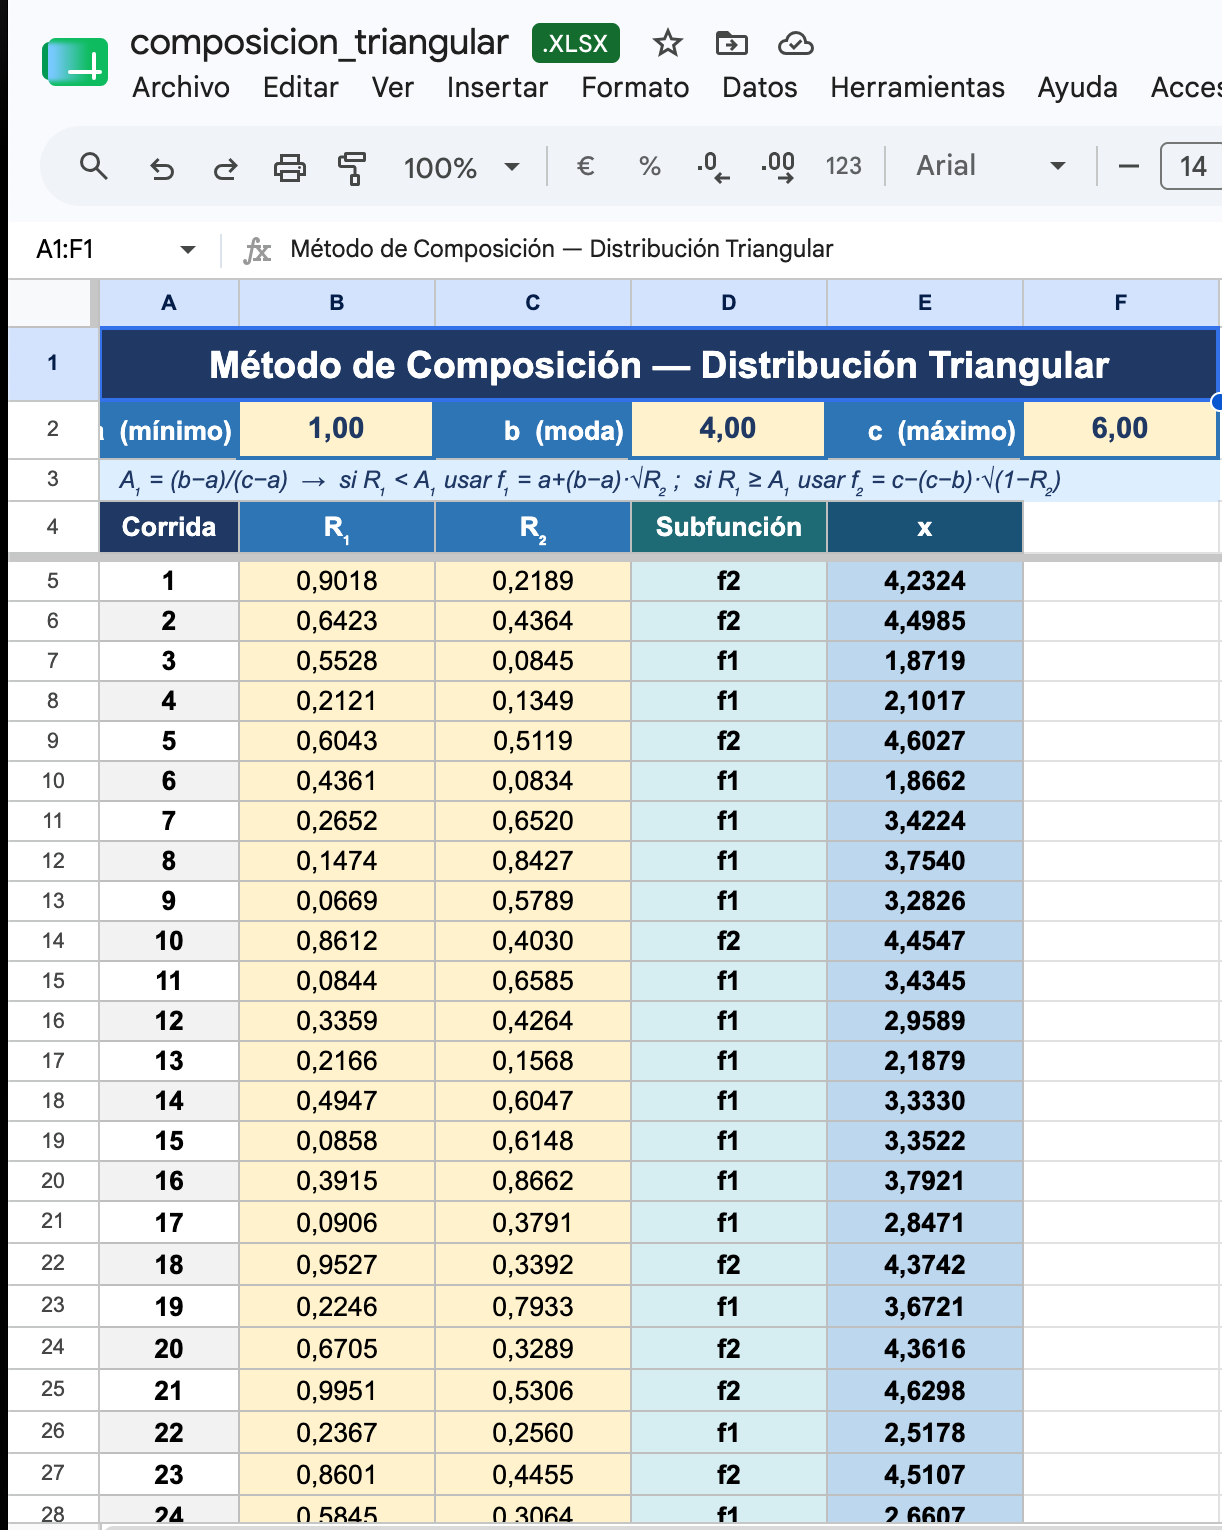
\includegraphics[width=0.9\textwidth]{capturas_excel/p2_composicion.png}
\caption{Hoja de cálculo — Composición}
\end{figure}

\subsection{Validación}

\subsubsection{\texorpdfstring{Prueba de escritorio con $n=25$}{Prueba de escritorio con n=25}}

\begin{mitabla}[H]{\texorpdfstring{Prueba de escritorio — $n=25$ corridas}{Prueba de escritorio - n=25 corridas}}
\small
\begin{tabular}{ccccc}
\toprule
Corrida & $R_1$ & $R_2$ & Sub & $x$ \\
\midrule
1  & 0,0360 & 0,8430 & $f_1$ & 3,7954 \\
2  & 0,3233 & 0,4009 & $f_1$ & 3,0830 \\
3  & 0,8452 & 0,6131 & $f_2$ & 4,9449 \\
4  & 0,8352 & 0,0089 & $f_2$ & 4,0111 \\
5  & 0,7362 & 0,4705 & $f_2$ & 4,6809 \\
6  & 0,9032 & 0,6130 & $f_2$ & 4,9448 \\
7  & 0,8695 & 0,6980 & $f_2$ & 5,1261 \\
8  & 0,4305 & 0,2852 & $f_1$ & 2,8351 \\
9  & 0,0885 & 0,3947 & $f_1$ & 3,0706 \\
10 & 0,3889 & 0,7682 & $f_1$ & 3,6912 \\
11 & 0,8191 & 0,8279 & $f_2$ & 5,4630 \\
12 & 0,4957 & 0,0343 & $f_1$ & 1,9631 \\
13 & 0,1853 & 0,6591 & $f_1$ & 3,5296 \\
14 & 0,9685 & 0,0592 & $f_2$ & 4,0751 \\
15 & 0,3201 & 0,6398 & $f_1$ & 3,4998 \\
16 & 0,6147 & 0,0361 & $f_2$ & 4,0456 \\
17 & 0,2580 & 0,0448 & $f_1$ & 2,0294 \\
18 & 0,2516 & 0,3752 & $f_1$ & 3,0314 \\
19 & 0,1156 & 0,9305 & $f_1$ & 3,9115 \\
20 & 0,6000 & 0,6125 & $f_2$ & 4,9437 \\
21 & 0,4884 & 0,2922 & $f_1$ & 2,8514 \\
22 & 0,3420 & 0,7870 & $f_1$ & 3,7178 \\
23 & 0,1244 & 0,3298 & $f_1$ & 2,9357 \\
24 & 0,9969 & 0,9364 & $f_2$ & 5,8694 \\
25 & 0,9680 & 0,3242 & $f_2$ & 4,4448 \\
\bottomrule
\end{tabular}
\end{mitabla}

$\bar{x}_{25} = 3{,}8598$

\subsubsection{\texorpdfstring{Corridas con $n \geq 50$}{Corridas con n mayor igual 50}}

\begin{mitabla}[H]{\texorpdfstring{Resumen de corridas con $n \geq 50$}{Resumen de corridas con n mayor igual 50}}
\begin{tabular}{cccc}
\toprule
$n$ & $\bar{x}$ & $x_{\min}$ & $x_{\max}$ \\
\midrule
50   & 4,2451 & 2,0906 & 5,9979 \\
100  & 4,1654 & 1,8410 & 6,0730 \\
250  & 4,0354 & 1,5589 & 6,3561 \\
500  & 3,9793 & 1,5922 & 6,3355 \\
1000 & 3,9964 & 1,7046 & 6,4485 \\
\bottomrule
\end{tabular}
\end{mitabla}

\subsection{Interpretación}

\subsubsection{Resultados}

En las 25 corridas de la prueba de escritorio, todos los valores de $x$ quedaron dentro del intervalo $[a,c]=[1{,}5,\,6{,}5]$ esperado, con media $\bar{x}_{25}=3{,}8598$, cercana al vértice $b=4$. Las corridas con $n \geq 50$ mantienen $x_{\min}$ y $x_{\max}$ dentro de $[a,c]$ y la media $\bar{x}$ se estabiliza progresivamente alrededor de $4{,}0$ conforme crece $n$.

\subsubsection{Interpretación}

Los resultados confirman que la selección de subfunción mediante $R_1$ y la aplicación de Transformada Inversa con $R_2$ generan correctamente valores de $x$ según la distribución triangular: la media se aproxima al vértice $b$ (moda de la triangular) y ningún valor generado cae fuera de $[a,c]$, lo cual es consistente con el modelo teórico planteado en la propuesta de solución.

\subsection{Conclusión}

El método de Composición permitió dividir la función triangular en dos subfunciones resueltas cada una por Transformada Inversa, seleccionadas mediante $R_1$ según la proporción de subáreas $A_1$ y $A_2$. La validación con prueba de escritorio (n=25 y $n \geq 50$) y la implementación en Java y Excel confirman que el modelo reproduce correctamente la distribución triangular esperada.


\newpage

\section{Control de Inventarios (sin espera del cliente)}

\subsection{Introducción}

Este problema corresponde a un \textbf{sistema de inventarios} con política de lote constante $q$ y punto de reorden $R$: cuando el nivel de inventario cae a $R$ o menos, se coloca una orden de $q$ unidades que tarda un tiempo de entrega aleatorio en llegar. Tanto la demanda diaria como el tiempo de entrega son variables aleatorias discretas dadas por tabla de probabilidad, por lo que la técnica aplicable es Transformada Inversa discreta (ver Ejemplo 4.4 de \texttt{Teorema.tex}), combinada con una simulación de eventos día a día del nivel de inventario, siguiendo el procedimiento del Ejemplo 5.5 (``Sistema de inventarios'') de Coss Bu.

\subsection{Descripción del problema}

La demanda diaria y el tiempo de entrega de un cierto producto, siguen las siguientes distribuciones de probabilidad:

\begin{center}
\begin{tabular}{cc}
\toprule
Demanda diaria & Probabilidad \\
\midrule
0 & 0.04 \\
1 & 0.06 \\
2 & 0.10 \\
3 & 0.20 \\
4 & 0.30 \\
5 & 0.18 \\
6 & 0.08 \\
7 & 0.03 \\
8 & 0.01 \\
\bottomrule
\end{tabular}
\qquad
\begin{tabular}{cc}
\toprule
Tiempo de entrega (días) & Probabilidad \\
\midrule
1 & 0.25 \\
2 & 0.50 \\
3 & 0.20 \\
4 & 0.05 \\
\bottomrule
\end{tabular}
\end{center}

La información con respecto a los costos relevantes es la siguiente:

\begin{itemize}
    \item Costo de ordenar: \$50/orden
    \item Costo de inventario: \$26/unidad/año
    \item Costo de faltante: \$25/unidad
\end{itemize}

Si el inventario inicial es de 15 unidades, ¿determine la cantidad óptima a ordenar (q) y el nivel óptimo de reorden (R)? (Asuma que se trabajan 260 días en el año.)

\subsection{Propuesta de solución}

\textbf{Demanda diaria}

\begin{description}
    \item[Paso 1: Encontrar la función $f(x)$]

    \begin{center}
    \begin{tabular}{cc}
    \toprule
    $x$ & $f(x)$ \\
    \midrule
    0 & 0.04 \\
    1 & 0.06 \\
    2 & 0.10 \\
    3 & 0.20 \\
    4 & 0.30 \\
    5 & 0.18 \\
    6 & 0.08 \\
    7 & 0.03 \\
    8 & 0.01 \\
    \bottomrule
    \end{tabular}
    \end{center}

    \item[Paso 2: Determinar la función acumulada $F(x)$]

    \begin{align*}
    F(0) &= f(0) = 0.04 \\
    F(1) &= F(0)+f(1) = 0.10 \\
    F(2) &= F(1)+f(2) = 0.20 \\
    F(3) &= F(2)+f(3) = 0.40 \\
    F(4) &= F(3)+f(4) = 0.70 \\
    F(5) &= F(4)+f(5) = 0.88 \\
    F(6) &= F(5)+f(6) = 0.96 \\
    F(7) &= F(6)+f(7) = 0.99 \\
    F(8) &= F(7)+f(8) = 1.00
    \end{align*}

    \item[Paso 3: Igualar la función acumulada $F(x) = R$]

    $$ F(x)=R \qquad ; \qquad 0 < R < 1 $$

    Se compara el $R$ generado contra la tabla de $F(x)$ hasta encontrar la primera fila donde $R < F(x)$.

    \item[Paso 4: Aplicar la función inversa $x=F^{-1}(R)$]

    \begin{center}
    \begin{tabular}{ll}
    Si $0.00 \leq R < 0.04$, entonces $x=0$ & Si $0.40 \leq R < 0.70$, entonces $x=4$ \\
    Si $0.04 \leq R < 0.10$, entonces $x=1$ & Si $0.70 \leq R < 0.88$, entonces $x=5$ \\
    Si $0.10 \leq R < 0.20$, entonces $x=2$ & Si $0.88 \leq R < 0.96$, entonces $x=6$ \\
    Si $0.20 \leq R < 0.40$, entonces $x=3$ & Si $0.96 \leq R < 0.99$, entonces $x=7$ \\
                                            & Si $0.99 \leq R \leq 1.00$, entonces $x=8$ \\
    \end{tabular}
    \end{center}

    \item[Paso 5: Propuesta algorítmica para la variable aleatoria]

    En vez de un \texttt{si/sino si} por cada valor, se guardan los valores y su acumulada en dos arreglos y se recorren con un bucle — sirve para cualquier tabla, sin importar su tamaño:

    \begin{lstlisting}[caption={demandaDiaria()}, language=Pascal]
valores   <- [0, 1, 2, 3, 4, 5, 6, 7, 8]
acumulada <- [0.04, 0.10, 0.20, 0.40, 0.70, 0.88, 0.96, 0.99, 1.00]

entero funcion demandaDiaria(){
    real R <- gcm();
    para i <- 0 hasta longitud(acumulada)-1 hacer
        si (R < acumulada[i]) entonces
            retornar valores[i];
        fin si
    fin para
}
    \end{lstlisting}
\end{description}

\textbf{Tiempo de entrega}

\begin{description}
    \item[Paso 1: Encontrar la función $f(x)$]

    \begin{center}
    \begin{tabular}{cc}
    \toprule
    $x$ (días) & $f(x)$ \\
    \midrule
    1 & 0.25 \\
    2 & 0.50 \\
    3 & 0.20 \\
    4 & 0.05 \\
    \bottomrule
    \end{tabular}
    \end{center}

    \item[Paso 2: Determinar la función acumulada $F(x)$]

    \begin{align*}
    F(1) &= f(1) = 0.25 \\
    F(2) &= F(1)+f(2) = 0.75 \\
    F(3) &= F(2)+f(3) = 0.95 \\
    F(4) &= F(3)+f(4) = 1.00
    \end{align*}

    \item[Paso 3: Igualar la función acumulada $F(x) = R$]

    $$ F(x)=R \qquad ; \qquad 0 < R < 1 $$

    \item[Paso 4: Aplicar la función inversa $x=F^{-1}(R)$]

    \begin{center}
    \begin{tabular}{l}
    Si $0.00 \leq R < 0.25$, entonces $x=1$ día \\
    Si $0.25 \leq R < 0.75$, entonces $x=2$ días \\
    Si $0.75 \leq R < 0.95$, entonces $x=3$ días \\
    Si $0.95 \leq R \leq 1.00$, entonces $x=4$ días \\
    \end{tabular}
    \end{center}

    \item[Paso 5: Propuesta algorítmica para la variable aleatoria]

    Misma idea: valores y acumulada en arreglos, bucle genérico:

    \begin{lstlisting}[caption={tiempoEntrega()}, language=Pascal]
valores   <- [1, 2, 3, 4]
acumulada <- [0.25, 0.75, 0.95, 1.00]

entero funcion tiempoEntrega(){
    real R <- gcm();
    para i <- 0 hasta longitud(acumulada)-1 hacer
        si (R < acumulada[i]) entonces
            retornar valores[i];
        fin si
    fin para
}
    \end{lstlisting}
\end{description}

\textbf{Lógica de simulación del inventario}

Con las dos variables anteriores ya definidas, cada día de la simulación sigue este orden: si llega un pedido programado para hoy, se suma $q$ al inventario; se genera la demanda del día; se resta del inventario (o se registra faltante si no alcanza); se registra el inventario promedio del día; y si el inventario queda en $R$ o menos sin pedido pendiente, se coloca una nueva orden. Los tres costos se calculan como:
\[
\text{Costo de ordenar} = (\text{n\'umero de \'ordenes}) \times \$50
\]
\[
\text{Costo de inventario} = \left(\sum \text{inventario promedio diario}\right) \times \frac{\$26}{260}
\]
\[
\text{Costo de faltante} = (\text{unidades faltantes}) \times \$25
\]
El par $(q,R)$ óptimo se encuentra probando distintos pares candidatos, simulando el costo total anual de cada uno (promediado sobre muchos años) y comparando.

\subsection{Objetivos}

\textbf{Objetivo general:} Aplicar Transformada Inversa discreta junto con simulación de eventos día a día para determinar la cantidad óptima a ordenar ($q$) y el punto de reorden ($R$) que minimizan el costo total anual del sistema de inventarios.

\textbf{Objetivos específicos:}
\begin{enumerate}
    \item Obtener las tablas de Transformada Inversa para la demanda diaria y el tiempo de entrega a partir de sus distribuciones de probabilidad.
    \item Simular el sistema de inventarios para distintos pares $(q, R)$ y comparar sus costos totales anuales para identificar el par óptimo.
\end{enumerate}

\subsection{Desarrollo de la solución}

\subsubsection{Algoritmo}

\begin{lstlisting}[caption={Simulación del sistema de inventarios}, language=Pascal]
real funcion simularInventario(entero q, entero R, entero dias){
    entero inventario, faltanteAcum, ordenes, diaLlegada, hayPedido;
    real sumaProm;

    inventario <- 15;
    faltanteAcum <- 0;
    ordenes <- 0;
    sumaProm <- 0;
    hayPedido <- falso;

    para dia <- 1 hasta dias hacer
        si (hayPedido) && (dia == diaLlegada) entonces
            inventario <- inventario + q;
            hayPedido <- falso;
        fin si

        invInicial <- inventario;
        demanda <- demandaDiaria();

        si (demanda <= inventario) entonces
            inventario <- inventario - demanda;
            promedioDia <- (invInicial + inventario) / 2;
        sino
            faltanteAcum <- faltanteAcum + (demanda - inventario);
            // El inventario se agota antes de terminar el dia: el promedio no es
            // (invInicial+0)/2, es el promedio de la parte con stock (invInicial/2)
            // multiplicado por la fraccion del dia que duro esa parte (invInicial/demanda),
            // igual que la Tabla 5.7 del Ejemplo 5.5.
            si (invInicial > 0) entonces
                promedioDia <- (invInicial / 2) * (invInicial / demanda);
            sino
                promedioDia <- 0;
            fin si
            inventario <- 0;
        fin si

        sumaProm <- sumaProm + promedioDia;

        si (inventario <= R) && (!hayPedido) entonces
            diaLlegada <- dia + tiempoEntrega();
            hayPedido <- verdadero;
            ordenes <- ordenes + 1;
        fin si
    fin para

    costoOrdenar <- ordenes * 50;
    costoInventario <- sumaProm * (26.0 / dias);
    costoFaltante <- faltanteAcum * 25;

    retornar costoOrdenar + costoInventario + costoFaltante;
}
\end{lstlisting}

\subsubsection{Diagrama de flujo}

\fbox{Pendiente}

\subsubsection{Tabla de simulación}

Simulación manual con $q=30$, $R=10$ (valores de partida, antes de optimizar) e inventario inicial de 15 unidades:

\begin{center}
\small
\begin{tabular}{cccccccc}
\toprule
\multirow{2}{*}{Día} & Inventario & Número & \multirow{2}{*}{Demanda} & Inventario & \multirow{2}{*}{Faltante} & \multirow{2}{*}{Orden} & Inventario \\
 & inicial & aleatorio & & final & & & diario promedio \\
\midrule
1  & 15 & 0.53 & 4 & 11 &   &   & 13.0 \\
2  & 11 & 0.81 & 5 & 6  &   & 1 & 8.5  \\
3  & 6  & 0.15 & 2 & 4  &   &   & 5.0  \\
4  & 34 & 0.68 & 4 & 30 &   &   & 32.0 \\
5  & 30 & 0.09 & 1 & 29 &   &   & 29.5 \\
6  & 29 & 0.77 & 5 & 24 &   &   & 26.5 \\
7  & 24 & 0.95 & 6 & 18 &   &   & 21.0 \\
8  & 18 & 0.31 & 3 & 15 &   &   & 16.5 \\
9  & 15 & 0.61 & 4 & 11 &   &   & 13.0 \\
10 & 11 & 0.98 & 7 & 4  &   & 2 & 7.5  \\
11 & 4  & 0.99 & 8 & 0  & 4 &   & 1.0  \\
12 & 0  & 0.45 & 4 & 0  & 4 &   & 0.0  \\
13 & 30 & 0.22 & 3 & 27 &   &   & 28.5 \\
\bottomrule
\end{tabular}
\end{center}

Orden 1 (día 2, $R=0.42$): tiempo de entrega $=2$ días, llega día 4. Orden 2 (día 10, $R=0.88$): tiempo de entrega $=3$ días, llega día 13.

El día 11 el inventario empieza en 4 pero la demanda es 8: no alcanza, y el inventario llega a 0 antes de terminar el día. El promedio de ese día no es $(4+0)/2$; es el promedio de la parte con stock ($4/2$) multiplicado por la fracción del día que duró esa parte ($4/8$), igual que la Tabla 5.7 del Ejemplo 5.5: $\text{promedio} = \frac{4}{2}\times\frac{4}{8}=1.0$. El día 12 el inventario ya empieza en 0, así que su promedio es directamente 0.

\begin{center}
\begin{tabular}{cccc}
\toprule
Costo de ordenar & Costo de inventario & Costo de faltante & Costo total \\
\midrule
$2(50)=\$100$ & $202.0(26/260)=\$20.20$ & $8(25)=\$200$ & \$320.20 \\
\bottomrule
\end{tabular}
\end{center}

\subsubsection{Implementación}

\begin{mitabla}[H]{Variables del modelamiento}
\begin{tabular}{cL{8cm}c}
\toprule
Variable & Descripción & Origen \\
\midrule
$q$ & Cantidad fija a ordenar en cada pedido & Variable de decisión \\
$R$ & Punto de reorden (nivel de inventario) & Variable de decisión \\
inventario & Estado del sistema, evoluciona día a día & Paso a paso \\
\bottomrule
\end{tabular}
\end{mitabla}

\begin{lstlisting}[caption={InventarioSimple.java}, language=Java]
import java.util.Random;

public class InventarioSimple {

    static Random rnd = new Random();

    // Tablas de Transformada Inversa: valores y su acumulada F(x).
    // El mismo generico() sirve para cualquier tabla, sin importar su tamaño.
    static final int[] VALORES_DEMANDA = {0, 1, 2, 3, 4, 5, 6, 7, 8};
    static final double[] ACUM_DEMANDA = {0.04, 0.10, 0.20, 0.40, 0.70, 0.88, 0.96, 0.99, 1.00};

    static final int[] VALORES_ENTREGA = {1, 2, 3, 4};
    static final double[] ACUM_ENTREGA = {0.25, 0.75, 0.95, 1.00};

    public static int generico(int[] valores, double[] acumulada) {
        double R = rnd.nextDouble();
        for (int i = 0; i < acumulada.length; i++) {
            if (R < acumulada[i]) {
                return valores[i];
            }
        }
        return valores[valores.length - 1];
    }

    public static int demandaDiaria() {
        return generico(VALORES_DEMANDA, ACUM_DEMANDA);
    }

    public static int tiempoEntrega() {
        return generico(VALORES_ENTREGA, ACUM_ENTREGA);
    }

    public static double simularInventario(int q, int R, int dias) {
        int inventario = 15;
        int faltanteAcum = 0;
        int ordenes = 0;
        boolean hayPedido = false;
        int diaLlegada = 0;
        double sumaProm = 0.0;

        for (int dia = 1; dia <= dias; dia++) {
            if (hayPedido && dia == diaLlegada) {
                inventario += q;
                hayPedido = false;
            }
            int invInicial = inventario;
            int demanda = demandaDiaria();
            double promedioDia;
            if (demanda <= inventario) {
                inventario -= demanda;
                promedioDia = (invInicial + inventario) / 2.0;
            } else {
                faltanteAcum += (demanda - inventario);
                // Igual que la Tabla 5.7 del Ejemplo 5.5: si el inventario se agota
                // antes de terminar el dia, el promedio es (invInicial/2)*(invInicial/demanda).
                promedioDia = (invInicial > 0) ? (invInicial / 2.0) * (invInicial / (double) demanda) : 0.0;
                inventario = 0;
            }
            sumaProm += promedioDia;
            if (inventario <= R && !hayPedido) {
                diaLlegada = dia + tiempoEntrega();
                hayPedido = true;
                ordenes++;
            }
        }
        double costoOrdenar = ordenes * 50.0;
        double costoInventario = sumaProm * (26.0 / dias);
        double costoFaltante = faltanteAcum * 25.0;
        return costoOrdenar + costoInventario + costoFaltante;
    }

    // Corre 13 dias imprimiendo cada paso del modelamiento (Paso 3: comparar R
    // contra F(x); Paso 4: tramo asignado), para verificar el codigo contra la
    // Propuesta de solucion.
    public static void demostracionModelamiento(int q, int R) {
        int inventario = 15;
        boolean hayPedido = false;
        int diaLlegada = 0;
        System.out.println("=== Demostracion del modelamiento (Pasos 3-4), q=" + q + " R=" + R + " ===");
        for (int dia = 1; dia <= 13; dia++) {
            if (hayPedido && dia == diaLlegada) {
                inventario += q;
                hayPedido = false;
                System.out.println("Dia " + dia + ": llega pedido, inventario += " + q);
            }
            int invInicial = inventario;
            double Rd = rnd.nextDouble();
            int demanda = 0;
            for (int i = 0; i < ACUM_DEMANDA.length; i++) {
                if (Rd < ACUM_DEMANDA[i]) { demanda = VALORES_DEMANDA[i]; break; }
                if (i == ACUM_DEMANDA.length - 1) demanda = VALORES_DEMANDA[i];
            }
            System.out.printf("Dia %d: R=%.4f (Paso 3: comparar contra F(x)) -> x=%d (Paso 4: demanda)%n",
                    dia, Rd, demanda);
            if (demanda <= inventario) {
                inventario -= demanda;
            } else {
                inventario = 0;
                System.out.println("  faltante = " + (demanda - invInicial));
            }
            System.out.println("  inventario: " + invInicial + " -> " + inventario);
            if (inventario <= R && !hayPedido) {
                double Re = rnd.nextDouble();
                int te = 0;
                for (int i = 0; i < ACUM_ENTREGA.length; i++) {
                    if (Re < ACUM_ENTREGA[i]) { te = VALORES_ENTREGA[i]; break; }
                    if (i == ACUM_ENTREGA.length - 1) te = VALORES_ENTREGA[i];
                }
                diaLlegada = dia + te;
                hayPedido = true;
                System.out.printf("  se ordena q=%d, R_entrega=%.4f -> tiempo=%d, llega dia %d%n",
                        q, Re, te, diaLlegada);
            }
        }
        System.out.println();
    }

    public static void main(String[] args) {
        demostracionModelamiento(30, 10);

        int mejorQ = 0, mejorR = 0;
        double mejorCosto = Double.MAX_VALUE;
        for (int q = 40; q <= 90; q += 2) {
            for (int R = 0; R <= 24; R += 2) {
                double suma = 0;
                for (int anio = 0; anio < 300; anio++) {
                    suma += simularInventario(q, R, 260);
                }
                double promedio = suma / 300;
                if (promedio < mejorCosto) {
                    mejorCosto = promedio;
                    mejorQ = q;
                    mejorR = R;
                }
            }
        }
        System.out.printf("Par optimo: q=%d, R=%d, costo promedio anual = %.2f%n",
                mejorQ, mejorR, mejorCosto);
    }
}
\end{lstlisting}

\textbf{Implementación en Excel:}

Hoja \texttt{P3\_InventarioSimple}. Datos de entrada en celdas fijas (\texttt{B1}=$q$, \texttt{B2}=$R$, \texttt{B3}=inventario inicial, \texttt{B4}=costo de ordenar, \texttt{B5}=costo de inventario, \texttt{B6}=costo de faltante). Las tablas de Transformada Inversa (demanda y tiempo de entrega) calculan $F(x)$ por suma acumulada de celdas (\texttt{=C(fila anterior)+B(fila actual)}), igual que en el Paso 2 de la propuesta de solución.

La tabla de simulación día a día usa, por fila: inventario final \texttt{=MAX(0;inicial-demanda)}, faltante \texttt{=MAX(0;demanda-inicial)}, inventario promedio con la corrección de la Tabla 5.7 cuando hay faltante \texttt{=SI(faltante=0;(inicial+final)/2;(inicial/2)*(inicial/demanda))}. Al final: costo de ordenar \texttt{=CONTAR.SI(columna\_orden;"Sí")*B4}, costo de inventario \texttt{=SUMA(columna\_promedio)*(B5/260)}, costo de faltante \texttt{=SUMA(columna\_faltante)*B6}. Una tabla de datos (Data Table) al costado prueba distintos pares $(q,R)$ y resalta el de menor costo total, coincidiendo con $q\approx60, R=12$.

\begin{figure}[H]
\centering
\fbox{\parbox{0.9\textwidth}{\centering\vspace{4cm}Captura de la hoja de cálculo — pendiente de agregar\vspace{4cm}}}
\caption{Hoja de cálculo — Control de Inventarios sin espera del cliente}
\end{figure}

\subsection{Validación}

\subsubsection{\texorpdfstring{Prueba de escritorio con $n=25$}{Prueba de escritorio con n=25}}

Costo total anual, corriendo la simulación completa (260 días) 25 veces con $q=60,R=12$:

\begin{center}
\small
\begin{tabular}{cccc}
\toprule
Corrida (año) & Costo total & Órdenes & Faltante \\
\midrule
1  & 1928.60 & 17 & 5 \\
2  & 1852.90 & 18 & 0 \\
3  & 1909.65 & 17 & 5 \\
4  & 1790.85 & 16 & 0 \\
5  & 1793.20 & 16 & 0 \\
6  & 1803.60 & 16 & 1 \\
7  & 1817.75 & 17 & 0 \\
8  & 1785.65 & 17 & 0 \\
9  & 1783.40 & 16 & 1 \\
10 & 1961.65 & 17 & 7 \\
11 & 1811.05 & 17 & 0 \\
12 & 1919.85 & 17 & 4 \\
13 & 1824.95 & 16 & 3 \\
14 & 1756.50 & 16 & 1 \\
15 & 1879.80 & 17 & 3 \\
16 & 1853.05 & 17 & 0 \\
17 & 1812.40 & 17 & 1 \\
18 & 1823.00 & 17 & 0 \\
19 & 1802.40 & 17 & 0 \\
20 & 1823.20 & 17 & 1 \\
21 & 1773.05 & 16 & 0 \\
22 & 1833.35 & 17 & 2 \\
23 & 1817.00 & 16 & 0 \\
24 & 1884.30 & 17 & 4 \\
25 & 1821.20 & 17 & 0 \\
\bottomrule
\end{tabular}
\end{center}

Promedio de las 25 corridas: \$1,834.49.

\subsubsection{\texorpdfstring{Corridas con $n \geq 50$}{Corridas con n mayor igual 50}}

\begin{center}
\begin{tabular}{cc}
\toprule
$n$ (años) & Costo total anual promedio \\
\midrule
50   & \$1,828.83 \\
100  & \$1,836.44 \\
250  & \$1,836.53 \\
500  & \$1,842.45 \\
1000 & \$1,840.40 \\
\bottomrule
\end{tabular}
\end{center}

El promedio se estabiliza alrededor de \$1,838 a medida que crece $n$, consistente con el resultado de la búsqueda de $(q,R)$.

\subsection{Interpretación}

\subsubsection{Resultados}

Probando pares $(q,R)$ candidatos (barrido con $q$ entre 40 y 90, $R$ entre 0 y 24, promediando 300 años simulados por par), el par de menor costo total anual promedio encontrado fue $q=64, R=12$ (Java) $/$ $q=59\text{--}65, R=12$ (verificado también en Python), con un costo total anual promedio de aproximadamente \textbf{\$1,838}. La zona alrededor de ese par es relativamente plana: varios valores de $q$ entre 57 y 65 con $R=12$ dan un costo muy similar (diferencias menores a \$10), mientras que $R=12$ es consistentemente mejor que $R=10$ o $R=14$ en esa zona.

En los días con faltante, el inventario promedio se calcula con la fórmula de la Tabla 5.7 del Ejemplo 5.5 (promedio de la parte con stock, ponderado por la fracción del día que duró) en vez del promedio simple entre inventario inicial y final, ya que el inventario se agota antes de terminar el día. Como los días con faltante son poco frecuentes con el par $(q,R)$ óptimo, su efecto sobre el costo total anual promedio es marginal.

\subsubsection{Interpretación}

El punto de reorden $R=12$ resulta mayor que la demanda esperada durante el tiempo de entrega ($\approx 3.7 \times 2.05 \approx 7.6$ unidades), lo cual es razonable: ese margen adicional (``inventario de seguridad'') reduce la frecuencia de faltantes sin disparar el costo de mantener inventario. La cantidad a ordenar $q \approx 60$ equivale a unas dos semanas de demanda esperada, lo cual balancea el costo de ordenar (menos órdenes si $q$ es grande) contra el costo de llevar inventario (más costo si $q$ es grande). Que la zona óptima sea plana significa que el sistema no es muy sensible a variaciones pequeñas de $q$ alrededor de 60, siempre que $R$ se mantenga cerca de 12.

\subsection{Conclusión}

El modelo de Transformada Inversa discreta combinado con la simulación día a día del inventario permitió determinar que la política óptima aproximada para este sistema es ordenar $q \approx 60$ unidades cada vez que el inventario cae a $R=12$ unidades o menos, con un costo total anual esperado de aproximadamente \$1,838. La validación con prueba de escritorio (n=25 y n$\geq$50) confirma que el algoritmo converge de forma estable a ese costo, y la implementación en Java reproduce el mismo resultado obtenido de forma independiente en la verificación con Python.


\newpage

\section{Control de Inventarios (con espera del cliente)}

\subsection{Introducción}

Este problema extiende el sistema de inventarios de p3 (política de lote constante $q$ y punto de reorden $R$) agregando una tercera variable aleatoria: el tiempo que un cliente está dispuesto a esperar cuando no hay stock disponible. Si el pedido en camino llega antes de que se cumpla ese plazo, la demanda pendiente se cubre (a un costo menor); si no, esa demanda se pierde definitivamente (a un costo mayor). Las tres variables (demanda diaria, tiempo de entrega, tiempo de espera) son discretas y se generan con Transformada Inversa, igual que en p3, sobre la misma lógica de simulación día a día del Ejemplo 5.5 (``Sistema de inventarios'') de Coss Bu.

\subsection{Descripción del problema}

La demanda diaria y el tiempo de entrega de un cierto producto, siguen las siguientes distribuciones de probabilidad:

\begin{center}
\begin{tabular}{cc}
\toprule
Demanda diaria & Probabilidad \\
\midrule
25 & 0.02 \\
26 & 0.04 \\
27 & 0.06 \\
28 & 0.12 \\
29 & 0.20 \\
30 & 0.24 \\
31 & 0.15 \\
32 & 0.10 \\
33 & 0.05 \\
34 & 0.02 \\
\bottomrule
\end{tabular}
\qquad
\begin{tabular}{cc}
\toprule
Tiempo de entrega (días) & Probabilidad \\
\midrule
1 & 0.20 \\
2 & 0.30 \\
3 & 0.25 \\
4 & 0.25 \\
\bottomrule
\end{tabular}
\end{center}

Si el producto no está disponible cuando es requerido, el cliente puede esperar la llegada de un nuevo lote por un tiempo limitado, es decir, si el cliente decide esperar 2 días y la mercancía no llega en ese tiempo, entonces, la demanda de este cliente se considera perdida. La distribución de probabilidad del tiempo que un cliente está dispuesto a esperar para que se le surta su pedido, es la siguiente:

\begin{center}
\begin{tabular}{cc}
\toprule
Tiempo de espera (días) & Probabilidad \\
\midrule
0 & 0.40 \\
1 & 0.20 \\
2 & 0.15 \\
3 & 0.15 \\
4 & 0.10 \\
\bottomrule
\end{tabular}
\end{center}

La información con respecto a los costos relevantes es la siguiente:

\begin{itemize}
    \item Costo de ordenar: \$100/orden
    \item Costo de inventario: \$52/unidad/año
    \item Costo de faltante suponiendo que el cliente espera: \$20/unidad
    \item Costo de faltante suponiendo que el cliente NO espera: \$50/unidad
\end{itemize}

Si el inventario inicial es de 100 unidades, ¿determine la cantidad óptima a ordenar (q) y el nivel óptimo de reorden (R)? (Asuma que se trabajan 260 días en el año.)

\subsection{Propuesta de solución}

\textbf{Demanda diaria}

\begin{description}
    \item[Paso 1: Encontrar la función $f(x)$]

    \begin{center}
    \begin{tabular}{cc}
    \toprule
    $x$ & $f(x)$ \\
    \midrule
    25 & 0.02 \\ 26 & 0.04 \\ 27 & 0.06 \\ 28 & 0.12 \\ 29 & 0.20 \\
    30 & 0.24 \\ 31 & 0.15 \\ 32 & 0.10 \\ 33 & 0.05 \\ 34 & 0.02 \\
    \bottomrule
    \end{tabular}
    \end{center}

    \item[Paso 2: Determinar la función acumulada $F(x)$]

    \begin{align*}
    F(25) &= f(25) = 0.02 \\
    F(26) &= F(25)+f(26) = 0.06 \\
    F(27) &= F(26)+f(27) = 0.12 \\
    F(28) &= F(27)+f(28) = 0.24 \\
    F(29) &= F(28)+f(29) = 0.44 \\
    F(30) &= F(29)+f(30) = 0.68 \\
    F(31) &= F(30)+f(31) = 0.83 \\
    F(32) &= F(31)+f(32) = 0.93 \\
    F(33) &= F(32)+f(33) = 0.98 \\
    F(34) &= F(33)+f(34) = 1.00
    \end{align*}

    \item[Paso 3: Igualar la función acumulada $F(x) = R$]

    $$ F(x)=R \qquad ; \qquad 0 < R < 1 $$

    \item[Paso 4: Aplicar la función inversa $x=F^{-1}(R)$]

    \begin{center}
    \begin{tabular}{ll}
    Si $0.00 \leq R < 0.02$, entonces $x=25$ & Si $0.44 \leq R < 0.68$, entonces $x=30$ \\
    Si $0.02 \leq R < 0.06$, entonces $x=26$ & Si $0.68 \leq R < 0.83$, entonces $x=31$ \\
    Si $0.06 \leq R < 0.12$, entonces $x=27$ & Si $0.83 \leq R < 0.93$, entonces $x=32$ \\
    Si $0.12 \leq R < 0.24$, entonces $x=28$ & Si $0.93 \leq R < 0.98$, entonces $x=33$ \\
    Si $0.24 \leq R < 0.44$, entonces $x=29$ & Si $0.98 \leq R \leq 1.00$, entonces $x=34$ \\
    \end{tabular}
    \end{center}

    \item[Paso 5: Propuesta algorítmica para la variable aleatoria]

    \begin{lstlisting}[caption={demandaDiaria()}, language=Pascal]
valores   <- [25, 26, 27, 28, 29, 30, 31, 32, 33, 34]
acumulada <- [0.02, 0.06, 0.12, 0.24, 0.44, 0.68, 0.83, 0.93, 0.98, 1.00]

entero funcion demandaDiaria(){
    real R <- gcm();
    para i <- 0 hasta longitud(acumulada)-1 hacer
        si (R < acumulada[i]) entonces
            retornar valores[i];
        fin si
    fin para
}
    \end{lstlisting}
\end{description}

\textbf{Tiempo de entrega}

\begin{description}
    \item[Paso 1: Encontrar la función $f(x)$]

    \begin{center}
    \begin{tabular}{cc}
    \toprule
    $x$ (días) & $f(x)$ \\
    \midrule
    1 & 0.20 \\ 2 & 0.30 \\ 3 & 0.25 \\ 4 & 0.25 \\
    \bottomrule
    \end{tabular}
    \end{center}

    \item[Paso 2: Determinar la función acumulada $F(x)$]

    \begin{align*}
    F(1) &= f(1) = 0.20 \\
    F(2) &= F(1)+f(2) = 0.50 \\
    F(3) &= F(2)+f(3) = 0.75 \\
    F(4) &= F(3)+f(4) = 1.00
    \end{align*}

    \item[Paso 3: Igualar la función acumulada $F(x) = R$]

    $$ F(x)=R \qquad ; \qquad 0 < R < 1 $$

    \item[Paso 4: Aplicar la función inversa $x=F^{-1}(R)$]

    \begin{center}
    \begin{tabular}{l}
    Si $0.00 \leq R < 0.20$, entonces $x=1$ día \\
    Si $0.20 \leq R < 0.50$, entonces $x=2$ días \\
    Si $0.50 \leq R < 0.75$, entonces $x=3$ días \\
    Si $0.75 \leq R \leq 1.00$, entonces $x=4$ días \\
    \end{tabular}
    \end{center}

    \item[Paso 5: Propuesta algorítmica para la variable aleatoria]

    \begin{lstlisting}[caption={tiempoEntrega()}, language=Pascal]
valores   <- [1, 2, 3, 4]
acumulada <- [0.20, 0.50, 0.75, 1.00]

entero funcion tiempoEntrega(){
    real R <- gcm();
    para i <- 0 hasta longitud(acumulada)-1 hacer
        si (R < acumulada[i]) entonces
            retornar valores[i];
        fin si
    fin para
}
    \end{lstlisting}
\end{description}

\textbf{Tiempo de espera del cliente (variable nueva respecto a p3)}

\begin{description}
    \item[Paso 1: Encontrar la función $f(x)$]

    \begin{center}
    \begin{tabular}{cc}
    \toprule
    $x$ (días) & $f(x)$ \\
    \midrule
    0 & 0.40 \\ 1 & 0.20 \\ 2 & 0.15 \\ 3 & 0.15 \\ 4 & 0.10 \\
    \bottomrule
    \end{tabular}
    \end{center}

    \item[Paso 2: Determinar la función acumulada $F(x)$]

    \begin{align*}
    F(0) &= f(0) = 0.40 \\
    F(1) &= F(0)+f(1) = 0.60 \\
    F(2) &= F(1)+f(2) = 0.75 \\
    F(3) &= F(2)+f(3) = 0.90 \\
    F(4) &= F(3)+f(4) = 1.00
    \end{align*}

    \item[Paso 3: Igualar la función acumulada $F(x) = R$]

    $$ F(x)=R \qquad ; \qquad 0 < R < 1 $$

    \item[Paso 4: Aplicar la función inversa $x=F^{-1}(R)$]

    \begin{center}
    \begin{tabular}{l}
    Si $0.00 \leq R < 0.40$, entonces $x=0$ días (no espera, se pierde de inmediato) \\
    Si $0.40 \leq R < 0.60$, entonces $x=1$ día \\
    Si $0.60 \leq R < 0.75$, entonces $x=2$ días \\
    Si $0.75 \leq R < 0.90$, entonces $x=3$ días \\
    Si $0.90 \leq R \leq 1.00$, entonces $x=4$ días \\
    \end{tabular}
    \end{center}

    \item[Paso 5: Propuesta algorítmica para la variable aleatoria]

    \begin{lstlisting}[caption={tiempoEspera()}, language=Pascal]
valores   <- [0, 1, 2, 3, 4]
acumulada <- [0.40, 0.60, 0.75, 0.90, 1.00]

entero funcion tiempoEspera(){
    real R <- gcm();
    para i <- 0 hasta longitud(acumulada)-1 hacer
        si (R < acumulada[i]) entonces
            retornar valores[i];
        fin si
    fin para
}
    \end{lstlisting}
\end{description}

\textbf{Lógica de simulación del inventario (con espera del cliente)}

La diferencia respecto a p3 está en qué pasa cuando la demanda supera el inventario disponible. Cada día, en este orden:
\begin{enumerate}
    \item Se revisan los ``pedidos en espera'' (backorders) cuyo plazo límite ya venció sin haber sido cubiertos: esas unidades se dan por perdidas (costo \$50/unidad).
    \item Si llega hoy un pedido, se suma $q$ al inventario, y ese inventario se usa primero para cubrir los pedidos en espera todavía vigentes (costo \$20/unidad cada una), antes de atender la demanda del día.
    \item Se genera la demanda del día. Si el inventario alcanza, se resta normalmente. Si no alcanza, la diferencia queda como faltante: se genera su tiempo de espera; si es 0 (40\% de probabilidad), se pierde de inmediato (\$50/unidad); si es mayor que 0, se guarda como pedido en espera con su plazo límite (día actual + tiempo de espera).
    \item Se registra el inventario promedio del día.
    \item Si el inventario queda en $R$ o menos y no hay pedido pendiente, se coloca una nueva orden.
\end{enumerate}

Los costos se calculan igual que en p3, agregando las dos tarifas de faltante:
\[
\text{Costo de ordenar} = (\text{n\'umero de \'ordenes}) \times \$100
\]
\[
\text{Costo de inventario} = \left(\sum \text{inventario promedio diario}\right) \times \frac{\$52}{260}
\]
\[
\text{Costo de faltante} = (\text{unidades cubiertas tras esperar}) \times \$20 + (\text{unidades perdidas}) \times \$50
\]
El par $(q,R)$ óptimo se encuentra probando distintos pares candidatos, simulando el costo total anual de cada uno (promediado sobre muchos años) y comparando, igual que en p3.

\subsection{Objetivos}

\textbf{Objetivo general:} Aplicar Transformada Inversa discreta (sobre demanda, tiempo de entrega y tiempo de espera) junto con simulación de eventos día a día para determinar la cantidad óptima a ordenar ($q$) y el punto de reorden ($R$) que minimizan el costo total anual del sistema de inventarios, considerando que el cliente puede esperar antes de que su demanda se pierda.

\textbf{Objetivos específicos:}
\begin{enumerate}
    \item Obtener las tablas de Transformada Inversa para la demanda diaria, el tiempo de entrega y el tiempo de espera del cliente.
    \item Simular el sistema de inventarios para distintos pares $(q, R)$, incorporando la lógica de pedidos en espera, y comparar sus costos totales anuales para identificar el par óptimo.
\end{enumerate}

\subsection{Desarrollo de la solución}

\subsubsection{Algoritmo}

\begin{lstlisting}[caption={Simulación del sistema de inventarios con espera del cliente}, language=Pascal]
real funcion simularInventario(entero q, entero R, entero dias){
    entero inventario, ordenes, diaLlegada, hayPedido;
    real sumaProm, costoEsperaOk, costoPerdida;
    lista backorders;  // cada elemento: (cantidad, plazoLimite)

    inventario <- 100;
    ordenes <- 0;
    sumaProm <- 0;
    costoEsperaOk <- 0;
    costoPerdida <- 0;
    hayPedido <- falso;

    para dia <- 1 hasta dias hacer
        para cada (cantidad, plazoLimite) en backorders hacer
            si (dia > plazoLimite) entonces
                costoPerdida <- costoPerdida + cantidad * 50;
                quitar (cantidad, plazoLimite) de backorders;
            fin si
        fin para

        si (hayPedido) && (dia == diaLlegada) entonces
            inventario <- inventario + q;
            hayPedido <- falso;
            para cada (cantidad, plazoLimite) en backorders hacer
                atendido <- minimo(cantidad, inventario);
                inventario <- inventario - atendido;
                costoEsperaOk <- costoEsperaOk + atendido * 20;
                actualizar cantidad restante en backorders;
            fin para
        fin si

        invInicial <- inventario;
        demanda <- demandaDiaria();

        si (demanda <= inventario) entonces
            inventario <- inventario - demanda;
            promedioDia <- (invInicial + inventario) / 2;
        sino
            faltante <- demanda - inventario;
            // Igual que en p3 (Tabla 5.7 del Ejemplo 5.5): si el inventario se agota
            // antes de terminar el dia, el promedio es (invInicial/2)*(invInicial/demanda).
            si (invInicial > 0) entonces
                promedioDia <- (invInicial / 2) * (invInicial / demanda);
            sino
                promedioDia <- 0;
            fin si
            inventario <- 0;
            espera <- tiempoEspera();
            si (espera == 0) entonces
                costoPerdida <- costoPerdida + faltante * 50;
            sino
                agregar (faltante, dia + espera) a backorders;
            fin si
        fin si

        sumaProm <- sumaProm + promedioDia;

        si (inventario <= R) && (!hayPedido) entonces
            diaLlegada <- dia + tiempoEntrega();
            hayPedido <- verdadero;
            ordenes <- ordenes + 1;
        fin si
    fin para

    costoOrdenar <- ordenes * 100;
    costoInventario <- sumaProm * (52.0 / dias);

    retornar costoOrdenar + costoInventario + costoEsperaOk + costoPerdida;
}
\end{lstlisting}

\subsubsection{Diagrama de flujo}

\fbox{Pendiente}

\subsubsection{Tabla de simulación}

Simulación manual con $q=90$, $R=40$ (valores de partida, antes de optimizar) e inventario inicial de 100 unidades. Se eligieron valores más ajustados que el óptimo para que se puedan observar ambos mecanismos de faltante (cobertura tras espera y pérdida definitiva):

\begin{center}
\small
\begin{tabular}{ccccccl}
\toprule
Día & Inv. inicial & Demanda & Inv. final & Faltante & Inv. promedio & Evento \\
\midrule
1  & 100 & 30 & 70  & --- & 85.0  & \\
2  & 70  & 26 & 44  & --- & 57.0  & \\
3  & 44  & 29 & 15  & --- & 29.5  & Ordena $q$=90 ($R_{ent}=0.22\Rightarrow$2 días), llega día 5 \\
4  & 15  & 31 & 0   & 16  & 3.63  & $R_{esp}=0.68\Rightarrow$espera 2 días, backorder hasta día 6 \\
5  & 74  & 32 & 42  & --- & 58.0  & Llega pedido (+90); cubre backorder 16u a \$20/u \\
6  & 42  & 27 & 15  & --- & 28.5  & Ordena $q$=90 ($R_{ent}=0.42\Rightarrow$2 días), llega día 8 \\
7  & 15  & 26 & 0   & 11  & 4.33  & $R_{esp}=0.22\Rightarrow$espera 0 días, \textbf{pierde} 11u a \$50/u \\
8  & 90  & 30 & 60  & --- & 75.0  & Llega pedido (+90) \\
9  & 60  & 26 & 34  & --- & 47.0  & Ordena $q$=90 ($R_{ent}=0.20\Rightarrow$1 día), llega día 10 \\
10 & 124 & 30 & 94  & --- & 109.0 & Llega pedido (+90) \\
11 & 94  & 30 & 64  & --- & 79.0  & \\
12 & 64  & 28 & 36  & --- & 50.0  & Ordena $q$=90 ($R_{ent}=0.59\Rightarrow$3 días), llega día 15 \\
13 & 36  & 31 & 5   & --- & 20.5  & \\
14 & 5   & 25 & 0   & 20  & 0.5   & $R_{esp}=0.81\Rightarrow$espera 3 días, backorder hasta día 17 \\
15 & 70  & 31 & 39  & --- & 54.5  & Llega pedido (+90); cubre backorder 20u a \$20/u; ordena de nuevo ($R_{ent}=0.34\Rightarrow$2 días), llega día 17 \\
16 & 39  & 28 & 11  & --- & 25.0  & \\
17 & 101 & 33 & 68  & --- & 84.5  & Llega pedido (+90) \\
18 & 68  & 29 & 39  & --- & 53.5  & Ordena $q$=90 ($R_{ent}=0.09\Rightarrow$1 día), llega día 19 \\
19 & 129 & 27 & 102 & --- & 115.5 & Llega pedido (+90) \\
20 & 102 & 32 & 70  & --- & 86.0  & \\
\bottomrule
\end{tabular}
\end{center}

Los días 4, 7 y 14 tienen faltante: el inventario se agota antes de terminar el día, así que su promedio usa la misma fórmula de la Tabla 5.7 del Ejemplo 5.5 que en p3 (por ejemplo, día 4: $\frac{15}{2}\times\frac{15}{31}=3.63$), no el promedio simple entre inicial y final.

En esta traza de 20 días se colocaron 6 órdenes, se cubrieron 36 unidades tras espera (16+20, a \$20/unidad) y se perdieron 11 unidades de inmediato (a \$50/unidad, porque el tiempo de espera generado fue 0). La suma de inventario promedio diario (columna de arriba) fue 1065.96.

\begin{center}
\begin{tabular}{cccc}
\toprule
Costo de ordenar & Costo de inventario & Costo de faltante & Costo total \\
\midrule
$6(100)=\$600$ & $1065.96(52/260)=\$213.19$ & $36(20)+11(50)=\$1{,}270$ & \$2{,}083.19 \\
\bottomrule
\end{tabular}
\end{center}

\subsubsection{Implementación}

\begin{mitabla}[H]{Variables del modelamiento}
\begin{tabular}{cL{8cm}c}
\toprule
Variable & Descripción & Origen \\
\midrule
$q$ & Cantidad fija a ordenar en cada pedido & Variable de decisión \\
$R$ & Punto de reorden (nivel de inventario) & Variable de decisión \\
inventario & Estado del sistema, evoluciona día a día & Paso a paso \\
backorders & Lista de faltantes en espera, con su plazo límite & Nuevo respecto a p3 \\
\bottomrule
\end{tabular}
\end{mitabla}

\begin{lstlisting}[caption={InventarioConEspera.java}, language=Java]
import java.util.ArrayList;
import java.util.List;
import java.util.Random;

public class InventarioConEspera {

    static Random rnd = new Random();

    static final int[] VALORES_DEMANDA = {25, 26, 27, 28, 29, 30, 31, 32, 33, 34};
    static final double[] ACUM_DEMANDA = {0.02, 0.06, 0.12, 0.24, 0.44, 0.68, 0.83, 0.93, 0.98, 1.00};

    static final int[] VALORES_ENTREGA = {1, 2, 3, 4};
    static final double[] ACUM_ENTREGA = {0.20, 0.50, 0.75, 1.00};

    static final int[] VALORES_ESPERA = {0, 1, 2, 3, 4};
    static final double[] ACUM_ESPERA = {0.40, 0.60, 0.75, 0.90, 1.00};

    public static int generico(int[] valores, double[] acumulada) {
        double R = rnd.nextDouble();
        for (int i = 0; i < acumulada.length; i++) {
            if (R < acumulada[i]) return valores[i];
        }
        return valores[valores.length - 1];
    }

    public static int demandaDiaria() { return generico(VALORES_DEMANDA, ACUM_DEMANDA); }
    public static int tiempoEntrega() { return generico(VALORES_ENTREGA, ACUM_ENTREGA); }
    public static int tiempoEspera()  { return generico(VALORES_ESPERA, ACUM_ESPERA); }

    static class Backorder {
        int cantidad;
        int plazoLimite;
        Backorder(int c, int p) { cantidad = c; plazoLimite = p; }
    }

    public static double simularInventario(int q, int R, int dias) {
        int inventario = 100;
        boolean hayPedido = false;
        int diaLlegada = 0;
        int ordenes = 0;
        double sumaProm = 0.0;
        double costoEsperaOk = 0.0;
        double costoPerdida = 0.0;
        List<Backorder> backorders = new ArrayList<>();

        for (int dia = 1; dia <= dias; dia++) {
            List<Backorder> vivos = new ArrayList<>();
            for (Backorder b : backorders) {
                if (dia > b.plazoLimite) costoPerdida += b.cantidad * 50.0;
                else vivos.add(b);
            }
            backorders = vivos;

            if (hayPedido && dia == diaLlegada) {
                inventario += q;
                hayPedido = false;
                List<Backorder> restantes = new ArrayList<>();
                for (Backorder b : backorders) {
                    if (inventario <= 0) { restantes.add(b); continue; }
                    int atendido = Math.min(b.cantidad, inventario);
                    inventario -= atendido;
                    costoEsperaOk += atendido * 20.0;
                    int resto = b.cantidad - atendido;
                    if (resto > 0) restantes.add(new Backorder(resto, b.plazoLimite));
                }
                backorders = restantes;
            }

            int invInicial = inventario;
            int demanda = demandaDiaria();
            double promedioDia;

            if (demanda <= inventario) {
                inventario -= demanda;
                promedioDia = (invInicial + inventario) / 2.0;
            } else {
                int faltante = demanda - inventario;
                // Igual que en p3 (Tabla 5.7 del Ejemplo 5.5): si el inventario se agota
                // antes de terminar el dia, el promedio es (invInicial/2)*(invInicial/demanda).
                promedioDia = (invInicial > 0) ? (invInicial / 2.0) * (invInicial / (double) demanda) : 0.0;
                inventario = 0;
                int te = tiempoEspera();
                if (te == 0) costoPerdida += faltante * 50.0;
                else backorders.add(new Backorder(faltante, dia + te));
            }

            sumaProm += promedioDia;

            if (inventario <= R && !hayPedido) {
                diaLlegada = dia + tiempoEntrega();
                hayPedido = true;
                ordenes++;
            }
        }

        double costoOrdenar = ordenes * 100.0;
        double costoInventario = sumaProm * (52.0 / dias);
        return costoOrdenar + costoInventario + costoEsperaOk + costoPerdida;
    }

    // Corre 20 dias imprimiendo cada paso del modelamiento (Paso 3: comparar R
    // contra F(x); Paso 4: tramo asignado) para las 3 variables (demanda, entrega,
    // espera), para verificar el codigo contra la Propuesta de solucion.
    public static void demostracionModelamiento(int q, int R) {
        int inventario = 100;
        boolean hayPedido = false;
        int diaLlegada = 0;
        List<Backorder> backorders = new ArrayList<>();

        System.out.println("=== Demostracion del modelamiento (Pasos 3-4), q=" + q + " R=" + R + " ===");
        for (int dia = 1; dia <= 20; dia++) {
            List<Backorder> vivos = new ArrayList<>();
            for (Backorder b : backorders) {
                if (dia > b.plazoLimite) {
                    System.out.println("Dia " + dia + ": vence backorder de " + b.cantidad + "u (costo $50 c/u)");
                } else {
                    vivos.add(b);
                }
            }
            backorders = vivos;

            if (hayPedido && dia == diaLlegada) {
                inventario += q;
                hayPedido = false;
                System.out.println("Dia " + dia + ": llega pedido, inventario += " + q);
                List<Backorder> restantes = new ArrayList<>();
                for (Backorder b : backorders) {
                    int atendido = Math.min(b.cantidad, inventario);
                    inventario -= atendido;
                    System.out.println("  cubre backorder " + atendido + "u (costo $20 c/u)");
                    int resto = b.cantidad - atendido;
                    if (resto > 0) restantes.add(new Backorder(resto, b.plazoLimite));
                }
                backorders = restantes;
            }

            int invInicial = inventario;
            double Rd = rnd.nextDouble();
            int demanda = 0;
            for (int i = 0; i < ACUM_DEMANDA.length; i++) {
                if (Rd < ACUM_DEMANDA[i]) { demanda = VALORES_DEMANDA[i]; break; }
                if (i == ACUM_DEMANDA.length - 1) demanda = VALORES_DEMANDA[i];
            }
            System.out.printf("Dia %d: R=%.4f (Paso 3: comparar contra F(x)) -> x=%d (Paso 4: demanda)%n",
                    dia, Rd, demanda);

            if (demanda <= inventario) {
                inventario -= demanda;
            } else {
                int faltante = demanda - inventario;
                inventario = 0;
                double Re = rnd.nextDouble();
                int te = 0;
                for (int i = 0; i < ACUM_ESPERA.length; i++) {
                    if (Re < ACUM_ESPERA[i]) { te = VALORES_ESPERA[i]; break; }
                    if (i == ACUM_ESPERA.length - 1) te = VALORES_ESPERA[i];
                }
                if (te == 0) {
                    System.out.printf("  faltante %du, R_espera=%.4f -> espera=0: PIERDE de inmediato ($50 c/u)%n", faltante, Re);
                } else {
                    backorders.add(new Backorder(faltante, dia + te));
                    System.out.printf("  faltante %du, R_espera=%.4f -> espera=%d dias, backorder hasta dia %d%n",
                            faltante, Re, te, dia + te);
                }
            }
            System.out.println("  inventario: " + invInicial + " -> " + inventario);

            if (inventario <= R && !hayPedido) {
                double Rt = rnd.nextDouble();
                int tent = 0;
                for (int i = 0; i < ACUM_ENTREGA.length; i++) {
                    if (Rt < ACUM_ENTREGA[i]) { tent = VALORES_ENTREGA[i]; break; }
                    if (i == ACUM_ENTREGA.length - 1) tent = VALORES_ENTREGA[i];
                }
                diaLlegada = dia + tent;
                hayPedido = true;
                System.out.printf("  se ordena q=%d, R_entrega=%.4f -> tiempo=%d, llega dia %d%n",
                        q, Rt, tent, diaLlegada);
            }
        }
        System.out.println();
    }

    public static void main(String[] args) {
        demostracionModelamiento(90, 40);

        int mejorQ = 0, mejorR = 0;
        double mejorCosto = Double.MAX_VALUE;
        for (int q = 130; q <= 230; q += 10) {
            for (int R = 90; R <= 140; R += 5) {
                double suma = 0;
                for (int anio = 0; anio < 400; anio++) {
                    suma += simularInventario(q, R, 260);
                }
                double promedio = suma / 400;
                if (promedio < mejorCosto) {
                    mejorCosto = promedio;
                    mejorQ = q;
                    mejorR = R;
                }
            }
        }
        System.out.printf("Par optimo: q=%d, R=%d, costo promedio anual = %.2f%n",
                mejorQ, mejorR, mejorCosto);
    }
}
\end{lstlisting}

\textbf{Implementación en Excel:}

Hoja \texttt{P4\_InventarioEspera}, misma estructura que p3, con datos de entrada distintos (\texttt{B1}=$q$=180, \texttt{B2}=$R$=115, \texttt{B3}=inventario inicial=100, \texttt{B4}=costo de ordenar=100, \texttt{B5}=costo de inventario=52, \texttt{B6}=costo de faltante con espera=20, \texttt{B7}=costo de faltante sin espera=50) y tres tablas de Transformada Inversa (demanda, entrega, espera) en vez de dos.

Como llevar varios pedidos en espera simultáneos con sus propios plazos límite es difícil con fórmulas nativas por fila, se usa una tabla auxiliar \texttt{Pendientes} al costado con columnas [Día del faltante, Cantidad, Día límite, Cubierto (Sí/No), Perdido (Sí/No)], una fila por cada evento de faltante, consultada desde la tabla principal con \texttt{BUSCARV}/\texttt{SUMAR.SI.CONJUNTO} para saber cuánto se cubre a \$20/unidad y cuánto se pierde a \$50/unidad. El resto (inventario promedio con la corrección de faltante, costo de ordenar, costo de inventario, búsqueda de $(q,R)$ óptimo) sigue la misma lógica que p3.

\begin{figure}[H]
\centering
\fbox{\parbox{0.9\textwidth}{\centering\vspace{4cm}Captura de la hoja de cálculo — pendiente de agregar\vspace{4cm}}}
\caption{Hoja de cálculo — Control de Inventarios con espera del cliente}
\end{figure}

\subsection{Validación}

\subsubsection{\texorpdfstring{Prueba de escritorio con $n=25$}{Prueba de escritorio con n=25}}

Costo total anual, corriendo la simulación completa (260 días) 25 veces con $q=180,R=115$:

\begin{center}
\small
\begin{tabular}{ccccc}
\toprule
Corrida (año) & Costo total & Órdenes & Unid. cubiertas tras espera & Unid. perdidas \\
\midrule
1  & 12208.70 & 44 & 0  & 0  \\
2  & 11809.90 & 43 & 23 & 0  \\
3  & 11738.00 & 44 & 10 & 0  \\
4  & 12008.20 & 43 & 2  & 0  \\
5  & 11653.90 & 44 & 0  & 4  \\
6  & 11926.60 & 44 & 0  & 0  \\
7  & 12653.20 & 43 & 26 & 7  \\
8  & 12421.80 & 44 & 0  & 0  \\
9  & 11503.60 & 43 & 9  & 0  \\
10 & 11807.80 & 44 & 1  & 0  \\
11 & 12107.10 & 43 & 0  & 6  \\
12 & 11375.60 & 43 & 0  & 0  \\
13 & 12175.60 & 43 & 26 & 4  \\
14 & 12555.80 & 43 & 1  & 11 \\
15 & 12041.20 & 43 & 0  & 3  \\
16 & 13476.90 & 44 & 0  & 26 \\
17 & 11823.00 & 44 & 1  & 0  \\
18 & 12027.20 & 44 & 34 & 2  \\
19 & 11904.80 & 44 & 2  & 3  \\
20 & 12328.10 & 44 & 9  & 0  \\
21 & 11826.10 & 44 & 0  & 1  \\
22 & 12198.40 & 44 & 18 & 0  \\
23 & 11629.50 & 44 & 0  & 0  \\
24 & 11774.10 & 43 & 6  & 0  \\
25 & 12289.90 & 44 & 0  & 5  \\
\bottomrule
\end{tabular}
\end{center}

Promedio de las 25 corridas: \$12,050.60.

\subsubsection{\texorpdfstring{Corridas con $n \geq 50$}{Corridas con n mayor igual 50}}

\begin{center}
\begin{tabular}{cc}
\toprule
$n$ (años) & Costo total anual promedio \\
\midrule
50   & \$12,040.52 \\
100  & \$12,125.76 \\
250  & \$12,118.61 \\
500  & \$12,099.73 \\
1000 & \$12,116.90 \\
\bottomrule
\end{tabular}
\end{center}

El promedio se estabiliza alrededor de \$12,100 a medida que crece $n$.

\subsection{Interpretación}

\subsubsection{Resultados}

Probando pares $(q,R)$ candidatos (barrido con $q$ entre 100 y 300, $R$ entre 90 y 180, refinado con 500 años simulados por par), el par de menor costo total anual promedio encontrado fue $q=180, R=115$, con un costo total anual promedio de aproximadamente \textbf{\$12,100}, verificado de forma independiente en Java ($q=180,R=115$, \$12{,}107) y Python ($q=180,R=115$, \$12{,}091). Igual que en p3, la zona alrededor de ese par es relativamente plana (pares entre $q=170$-$190$ con $R=115$ dan costos muy similares).

\subsubsection{Interpretación}

El punto de reorden $R=115$ es mayor que la demanda esperada durante el tiempo de entrega ($\approx 29.6 \times 2.05 \approx 60.7$ unidades), dejando un margen de seguridad considerable — mayor proporcionalmente que en p3, lo cual es razonable porque acá un faltante no siempre se pierde de inmediato (60\% de las veces el cliente espera), por lo que el sistema puede permitirse operar con algo más de holgura antes de que el costo de faltante se dispare. El costo total anual (\$12,100) es mucho mayor que el de p3 (\$1,838), lo cual es consistente con que la demanda diaria en p4 es casi 8 veces mayor (promedio $\approx 29.6$ contra $\approx 3.7$ unidades) y el costo de ordenar y de inventario también son más altos.

\subsection{Conclusión}

Incorporar la espera del cliente cambia la forma en que se contabiliza el faltante (dos tarifas en vez de una) pero no cambia la estructura general del modelo: sigue siendo Transformada Inversa discreta sobre las variables de entrada, combinada con simulación día a día del inventario. La política óptima aproximada encontrada es ordenar $q \approx 180$ unidades cada vez que el inventario cae a $R=115$ unidades o menos, con un costo total anual esperado de aproximadamente \$12,100. La validación con prueba de escritorio (n=25 y n$\geq$50) y la implementación independiente en Java y Python confirman que el modelo converge de forma estable a ese resultado.


\newpage

\section*{Bibliografía}
\addcontentsline{toc}{section}{Bibliografía}

\begin{itemize}
  \item Coss Bu, R. (1998). \textit{Simulación: un enfoque práctico}. Editorial Limusa, México.
\end{itemize}

\end{document}